\documentclass[12pt,italian,a4paper,oneside,openright]{book}
\usepackage{url,amsfonts,epsfig}
\usepackage[italian]{babel}
\usepackage[T1]{fontenc}
\usepackage[utf8]{inputenc}

%\usepackage[latin1]{inputenc}

%\usepackage[format=hang,font=footnotesize]{caption}
\usepackage{vmargin}
\usepackage{amsmath}
\usepackage{nccmath}
\usepackage{indentfirst}
\usepackage{graphicx}
\usepackage{listings}
\usepackage{lipsum}
\usepackage{tabularx}
\usepackage[table,dvipsnames]{xcolor}
\usepackage{multicol,booktabs,tabularx}
\usepackage{lipsum}
\usepackage{framed}
\usepackage{adjustbox}
\usepackage{empheq}
\usepackage[most]{tcolorbox}

% Per lo pseudocodice
\usepackage{algorithm}
\usepackage{algpseudocode}

\usepackage{ragged2e}

\makeatletter
\newenvironment{breakablealgorithm}
  {% \begin{breakablealgorithm}
   \begin{center}
     \refstepcounter{algorithm}% New algorithm
     \hrule height.8pt depth0pt \kern2pt% \@fs@pre for \@fs@ruled
     \renewcommand{\caption}[2][\relax]{% Make a new \caption
       {\raggedright\textbf{\fname@algorithm~\thealgorithm} ##2\par}%
       \ifx\relax##1\relax % #1 is \relax
         \addcontentsline{loa}{algorithm}{\protect\numberline{\thealgorithm}##2}%
       \else % #1 is not \relax
         \addcontentsline{loa}{algorithm}{\protect\numberline{\thealgorithm}##1}%
       \fi
       \kern2pt\hrule\kern2pt
     }
  }{% \end{breakablealgorithm}
     \kern2pt\hrule\relax% \@fs@post for \@fs@ruled
   \end{center}
  }
\makeatother

% Per il codice
\usepackage{xcolor}
\definecolor{codegreen}{rgb}{0,0.6,0}
\definecolor{codegray}{rgb}{0.5,0.5,0.5}
\definecolor{codepurple}{rgb}{0.58,0,0.82}
\definecolor{backcolour}{rgb}{0.95,0.95,0.92}

\lstdefinestyle{mystyle}{
    backgroundcolor=\color{white},   
    commentstyle=\color{codegreen},
    keywordstyle=\color{blue},
    numberstyle=\tiny\color{black},
    stringstyle=\color{codepurple},
    basicstyle=\ttfamily\footnotesize,
    breakatwhitespace=false,         
    breaklines=true,                 
    captionpos=b,                    
    keepspaces=true,                 
    numbers=left,                    
    numbersep=5pt,                  
    showspaces=false,                
    showstringspaces=false,
    showtabs=false,                  
    tabsize=2,
    otherkeywords={cudaError_t, size_t, __global__, __device__, dim3},
    frame=single
}

\lstset{style=mystyle}

%\usepackage{algorithm,algorithmic}
\graphicspath{{img/}}
\usepackage[hyperindex]{hyperref} %per l'indice interattivo
\hypersetup{colorlinks=true, linkcolor=black, urlcolor=blue, citecolor=blue} %per colorare i link
\DeclareGraphicsRule{.jpg}{jpg}{}{} %da commentare per il PDF
%\DeclareGraphicsRule{.bmp} {bmp}{}{} %da commentare per il PDF
\setmarginsrb{35mm}{30mm}{30mm}{30mm}{0mm}{10mm}{0mm}{10mm}
%%\setmarginsrb{1.5cm}{1.5cm}{1,2cm}{1,5cm}{0cm}{2cm}{2cm}{2cm}


\title{Template per la tesina in .tex}
\author{Nome e Cognome}
\date{Data di esame}

\begin{document}
\pagenumbering{Roman}

%%%% Opzione per interlinea 2
\baselineskip 1.5em

%% FRONTESPIZIO
{ \thispagestyle{empty}


\vskip 1cm \large \centerline{\textsc{\textbf{Universit\'a degli Studi di Napoli}}}
\large \centerline{\textsc{\textbf{``Parthenope''}}}

\vskip 0.5cm

\begin{center}

\includegraphics[scale=0.24]{logo_parthenope.png}
\end{center}

\centerline {\textsc{\textbf{Scuola interdipartimentale delle Scienze, dell'Ingegneria}}}
\centerline {\textsc{\textbf{e della Salute}}}

\vskip 0.5cm

\centerline {\textbf{Dipartimento di Scienze e Tecnologie}}

\vskip 0.5cm

\centerline {\textbf{Corso di laurea in Informatica}}

\vskip 0.5cm

\large \centerline {Tesi di laurea in Calcolo Parallelo e Distribuito}

\vskip 1.1cm

\Large \centerline {\textsc{\textbf{SIMULAZIONE NUMERICA SU GPU}}}
\Large \centerline{\textsc{\textbf{DI UN MODELLO DI VEGETAZIONE}}}

\vskip 1.1cm

\Large \centerline {\textsc{\textbf{NUMERICAL SIMULATION OF}}}
\Large \centerline {\textsc{\textbf{A VEGETATION MODEL ON GPU}}}

\vskip 1.1cm

\begin{minipage}[t]{7cm}
\normalsize \textsc{\textbf{Relatore:}}\\
Prof.ssa Livia Marcellino\\ \\
\normalsize \textsc{\textbf{Correlatore:}}\\
Prof. Pasquale De Luca
\end{minipage}
\hfill
\begin{minipage}[t]{5.5cm}
\normalsize \textsc{\textbf{Candidato:}}\\
Vincenzo Iannucci\\
Matricola 0124002093
\end{minipage}

\vskip 1.2 cm \Large \centerline {Anno Accademico 2021-2022}
\vfill \eject}

% fine frontespizio

\newpage 

\ % The empty page

\newpage

%%% DEDICA
%\thispagestyle{plain} \vspace*{\fill}
\begin{comment} ok \end{comment}
\noindent \textit{Ho deciso di dedicare questo spazio  dell’elaborato alle persone che mi sono state accanto nel corso del mio percorso di studi. In primis, un grazie speciale al mio relatore Livia Marcellino e correlatore Pasquale De Luca per gli indispensabili consigli e le conoscenze che mi hanno trasmesso durante la stesura della tesi. Ringrazio i miei compagni di corso Mario, Pasquale e Michele per aver condiviso parte del percorso universitario con me. Ringrazio i miei amici, Alessandro, Fabrizio, Attilio. In questi anni ho imparato a conoscervi e meglio e mi sono reso conto di quanto siete delle persone fantastiche e di quanto la nostra amicizia sia speciale. Grazie per avermi regalato momenti di allegria, emozione e condivisione indimenticabili, che mi porterò nel cuore per sempre. Un grazie speciale a Lorenzo, che con la sua dolcezza e pazienza mi ha insegnato ad essere meno melodrammatico e più sorridente. Il tuo sostegno mi è stato fondamentale in alcuni frangenti e questo non lo dimenticherò mai, sei una persona speciale. Grazie a mia madre e alla mia famiglia per aver accolto le mie scelte ed avermi sostenuto in tutti  questi anni, non sempre facili. Desidero inoltre dedicare questo lavoro alla memoria di mio nonno, che mi ha insegnato il valore dell'impegno e della determinazione. Anche se non è più con noi, so che sarebbe stato fiero di me per aver raggiunto questo traguardo. Mi sento in dovere di dedicare questo lavoro a chi purtroppo sempre più spesso decide di farla finita per aver fallito durante il percorso universitario. Se c’è una cosa che ho imparato è che la vita è un bene prezioso e non va sprecata a causa di uno o più fallimenti. Essi sono una naturale conseguenza della vita e vanno accettati, anche se a volte può risultare difficile e doloroso farlo. Con il tempo ho imparato che solo fallendo e cadendo in basso si può risalire ed arrivare in alto. Infine, grazie a me stesso, per non essermi arreso, per aver imparato dai fallimenti e per essere stato costante nello studio. Se sono arrivato fin qui oggi è anche merito delle tante notti insonni passate sui libri e dei sacrifici che ho fatto.}
\newpage

\renewcommand{\listalgorithmname}{Elenco degli algoritmi}

%\newpage
%\thispagestyle{plain}
\thispagestyle{headings}
\section*{Sommario}
\noindent Lo scopo della tesi è proporre uno schema parallelo per l'accelerazione di un algoritmo numerico che studia un problema di vegetazione in zone semiaride, modellato da un sistema di equazioni differenziali alle derivate parziali (PDE). Per farlo si è dapprima studiato il modello matematico proposto e la sua discretizzazione per il problema esposto. Successivamente, è stato formulato un algoritmo sequenziale che risolve il problema ed infine è stato implementato il software sequenziale. Dall'analisi delle prestazioni del software sequenziale e dalle successive osservazioni è stato progettato un algoritmo parallelo con una apposita strategia di parallelizzazione, che mira a calcolare contemporaneamente gli stage dell'equazione relativa alla discretizzazione temporale della PDE. Il software parallelo è stato implementato utilizzando l'ambiente CUDA per le GPU (Graphics Processing Unit) NVIDIA. La tesi è corredata di esperimenti numerici che mostrano il guadagno in termini di prestazioni della strategia proposta.

\section*{Abstract}
\noindent The purpose of the thesis is to propose a parallel scheme for the acceleration of a numerical algorithm that studies a vegetation problem in semi-arid areas, modeled by a system of Partial Differential Equation (PDE). To do that, the proposed mathematical model and its discretization for the problem  were first studied. Subsequently, a sequential algorithm that solves the problem was formulated and finally the sequential software was implemented. From the analysis of the performance of the sequential software and from the subsequent observations, a parallel algorithm was designed with a suitable parallelization strategy, which aims to simultaneously calculate the stages of the equation relating to the time discretization of the PDE. The parallel software was implemented using the CUDA environment for NVIDIA Graphics Processing Units (GPUs). Numerical experiments, showing the performance gain of the proposed strategy, are provided.

\thispagestyle{headings}
\chapter*{Introduzione} \label{cap:introduzione}

\noindent Il lavoro svolto si concentra sulla soluzione numerica efficiente di \textit{\textbf{PDE (Partial Differential Equation)}} che modellano un particolare problema di vegetazione, per mezzo di metodi numerici paralleli che utilizzano \textit{\textbf{GPU (Graphics Processing Unit)}}. 

\noindent Più precisamente, verrà preso in considerazione un sistema di PDE che rappresenta un modello di vegetazione in zone climatiche semi-aride, e costituisce un esempio del principio di autorganizzazione in ecologia. Tale sistema è stato introdotto per studiare come due specie erbacee competono per la stessa risorsa limitata (l'acqua) riuscendo a sopravvivere. \cite{bib:self-organization}

\noindent Per risolvere numericamente questo tipo di PDE, che è funzione spazio-tempo, è necessario discretizzare spazialemnte il problema generando così un sistema di \textit{\textbf{ODE (Ordinary Differential Equation)}}, che deve essere poi discretizzato rispetto al tempo. Una risoluzione efficiente prevede che il metodo impiegato non sia troppo costoso, cioè che coinvolga il minor numero possibile di valutazioni di funzioni e inversioni di matrici. Dunque, bisogna scegliere un metodo che sia numericamente stabile e non sia pesante computazionalmente. 

\noindent Un buon compromesso nella scelta del metodo di discretizzazione rispetto al tempo è rappresentato da una classe di metodi espliciti chiamati \textit{\textbf{peer methods}}. I peer methods sono metodi numerici basati su più passi (stage) che fanno parte della classe dei \textit{\textbf{General Linear Methods (GLM)}} \cite{general-linear-methods} 
%Sono più recenti dei metodi di Runge-Kutta
e hanno delle proprietà per cui il loro uso può risultare molto conveniente. Infatti, in questi metodi, tutte le fasi sono calcolate con la stessa accuratezza della soluzione che avanza, e questo assicura che i peer methods non soffrano di riduzione dell'ordine di accuratezza della soluzione finale.
%a differenza di quanto accade per i metodi Runge-Kutta \cite{runge-kutta-convergence}. 

\noindent L'attività svolta si è concentrata in primo luogo sulla scrittura di un algoritmo basato sul modello numerico che dati in input i parametri del modello restituisca in output la soluzione numerica del sistema \eqref{eq:main-equation}. Tale algoritmo è stato poi implementato in linguaggio di programmazione C, in un ambiente di calcolo sequenziale, organizzando l'algoritmo in più macromoduli.
\noindent Successivamente, si sono osservate le prestazioni del software e individuate le parti più critiche per cui fosse utile e necessario pensare ad una strategia di parallelizzazione. È stato quindi formulato un algoritmo parallelo, con relativa strategia di parallelizzazione, la quale mira proprio ad eseguire in parallelo i due stage (passi) dell'equazione relativa al calcolo dei peer methods. L'algoritmo parallelo è stato poi è stato implementato in ambiente ad alte prestazioni, sfruttando le architetture \textit{\textbf{GPU (Graphics Processing Units)}} e impiegando l'ambiente \textit{\textbf{CUDA}} \cite{cuda-environment}. 
Ricordiamo che oggigiorno la scelta delle GPU diventa quasi obbligatoria grazie alla possibilità che offrono di risolvere problemi di grandi dimensioni, mediante opportuni algoritmi paralleli, in un tempo di esecuzione ridotto.
Sono state usate le API in linguaggio C che CUDA mette a disposizione per la creazione del software parallelo. La scelta del linguaggio C è da ascriversi non solo al fatto che è stato ampiamente trattato durante il corso di studi ma anche al fatto che offre un controllo a basso livello della memoria, permettendo di utilizzare in maniera efficiente le risorse delle GPU. Infine, sono state analizzate e confrontate le performance osservando come il software parallelo abbia prestazioni nettamente migliori rispetto al sequenziale.

\noindent Il resto della tesi è organizzata come segue. Nel capitolo \ref{cap:modello-numerico} verrà presentato il problema di vegetazione, il modello matematico e i metodi di discretizzazione impiegati per passare al modello numerico. Verranno presentati in maniera più approfondita i peer methods e infine l'algoritmo sequenziale che risolve il problema di vegetazione. Il capitolo si conclude con i test effettuati sull'implementazione sequenziale dell'algoritmo. Nel capitolo \ref{cap:GPU} si parlerà delle GPU e dell'ambiente CUDA, con qualche esempio di codice in linguaggio C e una breve presentazione delle funzioni di libreria più usate. Nel capitolo \ref{cap:approccio-parallelo} si discuterà della strategia di parallelizzazione scelta e dell'algoritmo parallelo. Nel capitolo \ref{cap:test} verranno effettuati i test del codice parallelo e confrontati con i risultati ottenuti dalla controparte sequenziale, confermando l'efficienza dell'approccio parallelo.

\newpage
\markboth{Indice}{Indice}
\tableofcontents
\listoffigures
\listofalgorithms
\lstlistoflistings
\listoftables
\newpage

\pagenumbering{arabic}
\thispagestyle{headings}
\chapter{Un problema di vegetazione} \label{cap:modello-numerico}

\noindent Nel seguente capitolo verrà trattato un procedimento di discretizzazione che consente di passare dal modello matematico, che rappresenta il problema di vegetazione in esame, alla formulazione di un algoritmo per l'ambiente sequenziale e alla sua implementazione in ambiente CPU standard.

%%%%%%%%%%%%%%%%%%%%%%%%%%%%%%%%%%%%%%%%%%%%%%%%%%%%%%%%%%%%%%%
%              Il modello matematico
%%%%%%%%%%%%%%%%%%%%%%%%%%%%%%%%%%%%%%%%%%%%%%%%%%%%%%%%%%%%%%%
\section{Il modello matematico} \label{sec:math-model}
\noindent Consideriamo il seguente sistema di PDE:

\begin{equation}
    \begin{cases}
        \displaystyle
        \frac{\partial u_1}{\partial t} = \frac{\partial^2 u_1}{\partial x^2} + wu_1(u_1 + Hu_2) - B_1u_1 - Su_1u_2, \\\\
        \displaystyle
        \frac{\partial u_2}{\partial t} = D\frac{\partial^2 u_2}{\partial x^2} + Fwu_2(u_1 + Hu_2) - B_2u_2, \\\\
        \displaystyle
        \frac{\partial w}{\partial t} = d\frac{\partial^2 w}{\partial x^2} + A - w - w(u_1 + u_2)(u_1 + Hu_2). \\
    \end{cases}
    \label{eq:main-equation}
\end{equation}

\noindent Ove $(x, t) \in [x_0, X] \times [t_0, T]$, con le seguenti condizioni iniziali:
\begin{equation}
    \begin{cases}
        u_1(x, t_0) = U_{1, 0}(x),\\
        u_2(x, t_0) = U_{2, 0}(x),\\
        w(x, t_0) = W_0(x).
    \end{cases}
    \label{eq:main-equation-intial-condition}
\end{equation}

\noindent Esso rappresenta un modello di vegetazione in zone climatiche semi-aride ed è stato introdotto per studiare come due specie erbacee competono per la stessa risorsa limitata (l'acqua) riuscendo a sopravvivere. Per capire meglio come funziona il modello, si può immaginare che la funzione $u_1$ descriva la densità dell'erba presente sul suolo $x$ all'istante $t$, che la funzione $u_2$ rappresenti la stessa cosa ma per gli alberi, e che $w$ sia la quantità di acqua disponibile. La coesistenza delle due specie erbacee è uno stato metastabile, ovvero si presenta come soluzione stabile del sistema per tempi molto lunghi. Tuttavia, per $t \to \infty$ una delle due piante muore.

%%%%%%%%%%%%%%%%%%%%%%%%%%%%%%%%%%%%%%%%%%%%%%%%%%%%%%%%%%%%%%%
%              Discretizzazione spaziale
%%%%%%%%%%%%%%%%%%%%%%%%%%%%%%%%%%%%%%%%%%%%%%%%%%%%%%%%%%%%%%%
\section{Discretizzazione spaziale} \label{sec:space-semi-discretization}
\noindent Consideriamo l'equazione \eqref{eq:main-equation}. Il primo passo consiste nell'approssimare numericamente le derivate parziali rispetto allo spazio utilizzando il \textbf{MOL (Method Of Lines)}, che usando il metodo delle differenze finite centrali del secondo ordine (\textit{\textbf{central finite differences}}) permette di dividere l'intervallo spaziale $[x_0, X]$ in $M - 1$ sottointervalli:

\vspace{.5cm}

\begin{align*}
    \displaystyle
    \frac{\partial^2 u}{\partial x^2} = \frac{u(x + \Delta x,t) - 2u(x,t) + u(x - \Delta x,t)}{\Delta x^2}, \quad u = u_1, u_2, w, \quad \Delta x = \frac{X - x_0}{M - 1}
\end{align*}

\vspace{.5cm}

\noindent Dunque si passa da un sistema di PDE, costituito da derivate parziali e avente come variabili indipendenti il tempo e lo spazio ad un sistema di ODE, costituito da derivate ordinarie:

\begin{equation}
    \begin{cases}
        \displaystyle
        \frac{\partial U_1}{\partial t} = \frac{1}{\Delta x^2} L_{Diff}U_1 + F_1 \\\\
        \displaystyle
        \frac{\partial U_2}{\partial t} = \frac{D}{\Delta x^2} L_{Diff}U_2 + F_2 \\\\
        \displaystyle
        \frac{\partial W}{\partial t} = \frac{d}{\Delta x^2} L_{Diff}W + F_3 \\
    \end{cases}
    \label{eq:ODE-system}
\end{equation}

\noindent Per semplicità di notazione, è stata omessa la dipendenza dal tempo di tutte le funzioni coinvolte. La notazione usata è la seguente:

\begin{equation}
    \displaystyle
    x_m = x_0 + m \Delta x; \quad m = 0,\ldots, M - 1; \quad x_{M - 1} = X
    \label{eq:notations}
\end{equation}

\noindent e:

\begin{align*}
    u_1^m = u_1(x_m, t), \quad u_2^m = u_2(x_m, t), \quad w^m = w(x_m, t)
\end{align*} % end align
\begin{align*}
    U_1 = (u_1^m(t))^{M - 1}_{m = 0}, \quad U_2 = (u_2^m(t))^{M - 1}_{m = 0}, \quad W = (w^m(t))^{M - 1}_{m = 0}
\end{align*} % end align

\noindent con $U_1, U_2, W \in \mathbb{R}^{M}$.

\begin{align*}
    \frac{\partial U_1}{\partial t} = \Big( \frac{\partial u_1^m}{\partial t} \Big)_{m = 0}^{M - 1}, \quad \frac{\partial U_2}{\partial t} = \Big( \frac{\partial u_2^m}{\partial t} \Big)_{m = 0}^{M - 1}, \quad \frac{\partial W}{\partial t} = \Big( \frac{\partial w^m}{\partial t} \Big)_{m = 0}^{M - 1}
\end{align*} % end align
\begin{gather*}
    F_1 = (w^mu_1^m(u_1^m+Hu_2^m)-B_1u_1^m-Su_1^mu_2^m)^{M - 1}_{m = 0} \\
    F_2 = (Fw^mu_2^m(u_1^m+Hu_2^m)-B_2u_2^m)^{M - 1}_{m = 0} \\
    F_3 = (A - w^m - w^m(u_1^m+u_2^m)(u_1^m+Hu_2^m))^{M - 1}_{m = 0}
\end{gather*} % end gather

\noindent Al fine di completare la procedura di discretizzazione spaziale, se si assume che $u_1, u_2, w$ siano nulli al di fuori del loro dominio, risulta che la matrice $L_{Diff}$ è tridiagonale ed è data da:

\begin{equation}
    L_{Diff} = 
\begin{pmatrix}
    -2 & 1 & & & \\
    1 & -2 & 1 & \\
    & \ddots & \ddots & \ddots & & \\
    & & 1 & -2 & 1 \\
    & & & 1 & -2
 \end{pmatrix}
 \in \mathbb{R} ^ {M, M} \label{eq:matrix-Ldiff}
\end{equation}

\noindent Utilizzando condizioni al contorno periodiche, la matrice $L_{Diff}$ deve essere leggermente modificata, ponendo $L_{Diff}(1, M) = L_{Diff}(M, 1) = 1$. \\

\noindent Infine, compattando ulteriormente il sistema di ODE discrete \eqref{eq:ODE-system}, si ottiene:

\begin{equation}
    y'(t) = L \cdot y(t) + N L(y(t)) \label{eq:ODE-system-disc}
\end{equation}

\noindent dove:

\begin{equation}
    y(t) = [U_1, U_2, W]^T \in \mathbb{R} ^{3M} \ \text{ e } \ NL(y(t)) = [F_1, F_2, F_3]^T
    \label{eq:yt-system}
\end{equation}

\noindent mentre la matrice $L$ assume la forma:

\begin{equation}
    L = \frac{1}{\Delta x^2} 
\begin{pmatrix}
    L_{Diff} & 0 & 0 \\
    0 & DL_{Diff} & 0 \\
    0 & 0 & dL_{Diff}
 \end{pmatrix}
 \in \mathbb{R} ^ {3M, 3M} \label{eq:matrix-L}.
\end{equation}

\noindent Il passo successivo mira a discretizzare il sistema di ODE \eqref{eq:ODE-system-disc} mediante peer methods.

%%%%%%%%%%%%%%%%%%%%%%%%%%%%%%%%%%%%%%%%%%%%%%%%%%%%%%%%%%%%%%%
%     Discretizzazione rispetto al tempo con peer methods
%%%%%%%%%%%%%%%%%%%%%%%%%%%%%%%%%%%%%%%%%%%%%%%%%%%%%%%%%%%%%%%
\section{Discretizzazione rispetto al tempo con peer methods} \label{sec:time-discretization}
\noindent L'equazione (\ref{eq:ODE-system-disc}) rappresenta un sistema di ODE in forma vettoriale. Per discretizzare rispetto al tempo il sistema di ODE si può fare affidamento su due tipi principali di metodi: \textbf{espliciti} e \textbf{impliciti}. Nei metodi espliciti, la soluzione al passo temporale successivo viene stimata direttamente dai valori della soluzione al passo temporale corrente. Nei metodi impliciti, la soluzione al passo temporale successivo viene stimata risolvendo un'equazione non lineare che coinvolge sia il passo temporale corrente che quello successivo.
La scelta del metodo di discretizzazione temporale \textbf{dipende dal problema specifico da risolvere}, nonché dal compromesso desiderato tra accuratezza ed efficienza computazionale. \noindent Per risolvere il sistema di ODE sarebbe preferibile utilizzare un metodo che non sia troppo costoso, cioè che coinvolga il minor numero possibile di valutazioni di funzioni e inversioni di matrici. Dunque, bisogna scegliere un metodo che sia numericamente stabile e non sia pesante computazionalmente. \noindent Di solito si fa uso di metodi impliciti come quello di \textit{\textbf{Runge-Kutta}} \cite{implicit-runge-kutta, implicit-runge-kutta-2}, Rosenbrock o IMEX.
\noindent Tuttavia i metodi implici richiedono ad ogni passo di integrazione e per ogni stage di calcolare un sistema di equazioni lineari o non lineari, che richiedono di eseguire numericamente delle inversioni di matrici la cui dimensione è proporzionale alla dimensione del problema. Dunque, i metodi impliciti sono sì costosi ma sono gli unici che soddisfano i requisiti di stabilità richiesti dal problema. D'altro canto, i metodi espliciti non comportano la risoluzione di sistemi di equazioni, ma richiedono di usare un intervallo temporale molto piccolo e per questo motivo tali metodi impiegano un tempo considerevolmente elevato per convergere.
Un buon compromesso tra accuratezza ed efficienza computazionale è rappresentato da una classe di metodi espliciti denominata \textbf{peer methods} [\cite{peer-methods-1}-\cite{peer-methods-10}].
I peer methods sono una classe di metodi numerici basati su più passi (stage) che risolvono sistemi di ODE del primo ordine, nella forma generale di Cauchy $y(t) = f(t,y(t)) (t \in [t_0,T])$ con condizione iniziale $y_0 = y(t_0) \in \mathbb{R}^d$. Si consideri la discretizzazione temporale:

\begin{equation}
    t_n = t_0 + nh; \quad n = 0, \ldots, N; \quad t_N = T 
\end{equation}

\noindent dell'intervallo di integrazione $[t_0,T]$ relativo alla \eqref{eq:main-equation}, e quindi alla \eqref{eq:ODE-system-disc}. I peer methods basati su stage, espliciti, con $s$-stage e con dimensione del passo fissa $h$, hanno la seguente forma:

\begin{equation}
    Y_{n, i} = \sum_{j = 1}^s b_{ij}Y_{n - 1, j} + h\sum_{j = 1}^s a_{ij} f(t_{n - 1, j}, Y_{n - 1, j}), \quad n = 0,\ldots, N - 1
    \label{eq:peer-methods-1}
\end{equation}
\begin{gather*}
    Y_{n, i} \approx y(t_{n, i}), \qquad t_{n, i} = t_n + hc_i \qquad i = 1, \ldots, s.
\end{gather*}

\noindent dove $c_i$ sono i nodi in $[0, 1]$. Quindi, la soluzione progressiva $Y_{n,s}$ è l'approssimazione numerica di $y(t_n +h)$, cioè l'ultima fase calcola la soluzione numerica nei punti della griglia. I coefficienti nelle matrici $A = (a_{ij})^s _{i,j=1}$ e $B = (b_{ij})^s_{i,j=1}$ caratterizzano il peer methods utilizzato. Per scegliere i coefficienti delle matrici dobbiamo richiamare qualche risultato teorico. Per prima cosa, i peer methods si dicono ottimisticamente zero stabili imponendo:

\begin{equation*}
    (b_{ij})^{s-1}_{i,j=1} = 0, \qquad \text{ e } \qquad b_{is} = 1, \forall i = 1, \ldots, s.
\end{equation*}

\noindent Questa scelta è legata alla stabilità dei peer methods vicino all'origine \cite{two-step-peer-methods}. Inoltre, i coefficienti della matrice $A$ vengono assegnati imponendo l'ordine di consistenza dei peer methods \cite{two-step-peer-methods}, ovvero annullando un numero necessario di residui, definiti come:

\begin{equation*}
    h\Delta_i := y(t_{n,i}) - \sum_{j = 1}^{s}b_{ij}y(t_{n-1,j}) - h\sum_{j = 1}^{s}a_{ij}y'(t_{n-1,j}), \qquad i = 1,\ldots,s.
\end{equation*}

\noindent dove $y$ si estende su opportune basi polinomiali. Si noti che l'$i$-esimo residuo misura l'errore tra l'$i$-esimo stage e il suo valore esatto. Quindi, assumendo peer methods a $s$-stage di ordine $p = s$, i coefficienti $(a_{ij})^s_{i,j=1}$ devono soddisfare la relazione \cite{two-step-peer-methods}:

\begin{equation*}
    A = (CV_0D^{-1})V_1^{-1}-B(C-I_s)V_1D^{-1}V_1^{-1}
\end{equation*}

\noindent dove $V_0 = (c_i^{j - 1})^s_{i,j=1},  V_1 = ((c_i-1)^{j - 1})^{s}_{i,j=1}, C=diag(c_i), D = diag(1, \ldots, s)$ e $I_s$ è la matrice identità di dimensione $s$. In particolare, nello schema proposto, si sceglie di utilizzare i valori per $s = 2$ per quanto riguarda il numero di stage. Con queste condizioni, otteniamo:

\begin{equation}
    A = 
    \begin{pmatrix}
        0 & 0 \\
        -1/2 & 3/2
    \end{pmatrix},
    \quad
    B = 
    \begin{pmatrix}
        0 & 1 \\
        0 & 1
    \end{pmatrix},
    \quad
    (c_1, c_2) = (0, 1)
    \label{eq:ABc-equation}
\end{equation}

\noindent per $s = 2$.

\noindent Indicando con $\mathcal{F}$ le valutazioni delle funzioni degli stage in ogni punto discreto $t_{n,i}$, cioè,

\begin{gather*}
    \mathcal{F}(Y^{[n]})=(f(t_{n,1}, Y_{n,1})) \\
    \mathcal{F}(Y^{[n]})=(f(t_{n,2}, Y_{n,2})) 
\end{gather*}

\noindent è possibile rappresentare i peer methods \eqref{eq:peer-methods-1} in forma vettoriale:

\begin{equation}
    Y^{[n]} = (B \otimes I_d)Y^{[n - 1]} + h(A \otimes I_d) \mathcal{F}(Y^{[n - 1]})
    \label{eq:vector-representation-peer-methods}
\end{equation}

\noindent dove $d$ la dimensione della soluzione e $I_d$ è la matrice identità di ordine $d$. Infine, possiamo derivare l'intera procedura numerica ponendo nella formula \eqref{eq:vector-representation-peer-methods} $d = 3M$ e:

\begin{gather}
    \mathcal{F}(Y^{[n - 1]}) = (LY_{n - 1,1}+NL(Y_{n - 1,1})) \nonumber \\
    \mathcal{F}(Y^{[n - 1]}) = (LY_{n - 1,2}+NL(Y_{n - 1,2}))
    \label{eq:FYnm1-equation}
\end{gather}

\noindent dove $L$ e $NL$ sono come in \eqref{eq:yt-system} e \eqref{eq:matrix-L}, e applicando lo schema al problema di vegetazione nella forma ODE \eqref{eq:ODE-system-disc}. \\
\noindent Per capire meglio come i peer methods possono essere implementati prima in sequenziale e poi in parallelo, li si può riscrivere in maniera più estesa come segue:

\NewEnviron{NORMAL}{% 
    \scalebox{2}{$\BODY$} 
} 
 
\NewEnviron{HUGE}{% 
    \scalebox{5}{$\BODY$} 
}

\begin{gather}
    Y_{n,1} = b_{11}Y_{n-1, 1} + \ldots + b_{1s}Y_{n-1, s} + ha_{11}f(t_{n-1, 1}, Y_{n-1,1}) +  \ldots + ha_{1s}f(t_{n-1, s}, Y_{n-1,s}),\nonumber\\
    Y_{n,2} = b_{21}Y_{n-1, 1} + \ldots + b_{2s}Y_{n-1, s} + ha_{21}f(t_{n-1, 1}, Y_{n-1,1}) +  \ldots + ha_{2s}f(t_{n-1, s}, Y_{n-1,s}). \nonumber\\
    \label{eq:extended-peer-methods}
\end{gather}

\noindent Da questa scrittura risulta evidente che tutti gli stage nell'intervallo $[t_n, t_n + h]$ sono funzione di tutti gli stage nell'intervallo $[t_{n} - h, t_{n}]$. Quindi la soluzione progressiva $y(t_n + h) \approx Y_{n,s}$.

%%%%%%%%%%%%%%%%%%%%%%%%%%%%%%%%%%%%%%%%%%%%%%%%%%%%%%%%%%%%%%%
%                   Algoritmo sequenziale
%%%%%%%%%%%%%%%%%%%%%%%%%%%%%%%%%%%%%%%%%%%%%%%%%%%%%%%%%%%%%%%
\section{Algoritmo sequenziale} \label{sec:approccio-sequenziale}
\noindent Le discussioni precedenti ci consentono di introdurre un algoritmo che richiama i principali passaggi numerici sopra descritti.
L'algoritmo \ref{alg:peerMethodsSequential} mostra le operazioni necessarie per trovare la soluzione numerica del problema descritto, basata sulla discretizzazione discussa precedentemente.

\newpage

%--------------------------------------------------------------
%                   Algoritmo sequenziale
%--------------------------------------------------------------
\vspace{0.2cm}
\begin{breakablealgorithm}
    \caption{Algoritmo sequenziale peer methods}\label{alg:peerMethodsSequential}
    \vspace{0.5cm}
    \textbf{Input} $s,x_0,X,N, t_0, T,M, y_0, a,B_1,B_2,H, F, S, d, D, k, \Delta t$. \quad
    \textbf{Output} $Y$
    \vspace{0.2cm}
    \begin{algorithmic}[1]
        \Statex \textbf{// Initialization}
        \State $t\_span = [t_0, T]$
        \State time discretization $t_n(n = 0, \ldots, N)$
        \State $N = (t\_span[2]-t\_span[1])/\Delta t$
        \State $x\_span = [x_0, X]$
        \State space discretization $x_m(m = 0, \ldots, M - 1)$
        \State $\Delta x = (x\_span[2]-x\_span[1])/(M - 1)$
        \Statex \textbf{// Spatial discretization}
        \State defineLMatrix($L, \Delta x$)
        \Statex \textbf{// Time discretization by peer methods}
        \State $s = 2$ // set the number of stages
        \Statex // Initialization with time step $n = 0$
        \State \texttt{set} $t_{0,1} = t_0 + h \cdot c_1$
        \State \texttt{set} $t_{0,2} = t_0 + h \cdot c_2$
        \State \texttt{compute} $Y_{0,1}$ and $Y_{0,2}$ using Runge-Kutta 4th order method
        \State \texttt{evaluate} $\mathcal{F}((Y_{0,1}))$ and $\mathcal{F}((Y_{0,2}))$ as in \eqref{eq:FYnm1-equation}
        \Statex // Main loop: loop on time steps
        \For {$n = 1, \ldots, N$} 
        \State \texttt{set} $t_{n,1} = t_n + h \cdot c_1$
        \State \texttt{set} $t_{n,2} = t_n + h \cdot c_2$
        \State \texttt{compute} $Y_{n,1}$ and $Y_{n,2}$ as in \eqref{eq:extended-peer-methods}
        \State \texttt{evaluate} $\mathcal{F}((Y_{n,1}))$ and $\mathcal{F}((Y_{n,2}))$ as in \eqref{eq:FYnm1-equation}
        \EndFor
    \end{algorithmic}
\end{breakablealgorithm}
\vspace{0.2cm}
%--------------------------------------------------------------
%                Spiegazione pseudocodice
%--------------------------------------------------------------
\begin{itemize}
    \item \texttt{Righe 2-7}: l'algoritmo inizializza i parametri necessari per la discretizzazione del tempo e dello spazio. I parametri iniziali sono:
    \begin{itemize}
        \item $t_0$ tempo iniziale;
        \item $T$ tempo finale;
        \item $x_0$ spazio iniziale;
        \item $X$ spazio finale;
        \item $M$ dimensione della griglia spaziale;
        \item $N$ dimensione della griglia temporale;
        \item $k$ indice che rappresenta la $k$-esima diagonale, se posto a 0 rappresenta la diagonale principale;
        \item $\Delta t$ distanza tra un valore e l'altro dell'intervallo temporale discretizzato;
        \item $s$ numero di stage;
        \item a, $B_1$, $B_2$, H, F, S parametri di $NL(y(t))$ dell'equazione (\ref{eq:ODE-system-disc});
        \item d, D parametri di $L \cdot y(t)$ dell'equazione (\ref{eq:ODE-system-disc}).
    \end{itemize}
    \item \texttt{Riga 9}: \texttt{defineLMatrix} rappresenta il primo macro-modulo dell'algoritmo sequenziale. Per discretizzare rispetto alla coordinata spaziale, dobbiamo definire la matrice tridiagonale a blocchi $L$ \eqref{eq:matrix-L} come segue:
    \begin{enumerate}
        \item Definire la matrice identità \texttt{eye} di dimensione $M \times M$
        \item Definire due matrici $M \times M$ con la $k + 1$ e $k - 1$ diagonale unitaria, dove $k = 0$ rappresenta la diagonale principale.
        \item Sommare le tre matrici calcolate ai passi precedenti per ottenere la matrice $L_{Diff}$ \eqref{eq:matrix-Ldiff}
        \item Impostare $L_{Diff} (M,1) = L_{Diff} (1,M) = 1$
        \item Moltiplicare la matrice $L_{Diff}$ per $1 / \Delta x^2$
        \item Moltiplicare $L_{Diff}$ rispettivamente per gli scalari $D$ e $d$ \eqref{eq:init-parameters} passati in input, ottenendo le matrici $DL_{Diff}$ e $dL_{Diff}$
        \item Costruire la matrice tridiagonale a blocchi $L$ avente sulla diagonale principale le matrici $L_{Diff}$, $DL_{Diff}$ e $dL_{Diff}$
    \end{enumerate}
    \item \texttt{Righe 11-22}: dopo aver discretizzato rispetto la coordinata spaziale adesso non ci resta che discretizzare rispetto al tempo grazie all'utilizzo dei peer methods. Per prima cosa si calcola il valore di $Y$ quando $n = 0$ e per tutti gli stage $s$, ossia $Y_{0, i} \quad (i = 1 \ldots s)$, usando il metodo esplicito ad un passo di Runge-Kutta del quarto ordine, che garantisce che il peer methods mantenga lo stesso ordine di accuratezza quando calcola il successivo valore $Y_{n, i}$. Successivamente, per poter applicare l'equazione \eqref{eq:peer-methods-1} e quindi \eqref{eq:vector-representation-peer-methods}, bisogna definire la funzione $\mathcal{F}(Y^{[n]})$ come in \eqref{eq:FYnm1-equation}. Al passo $n + 1$, questa funzione diverrà $\mathcal{F}(Y^{[n - 1]})$ e potrà essere usata nella formula del peer methods. Infatti alle righe \texttt{18-22} si trova il loop principale del metodo, che altro non fa che eseguire le stesse operazioni eseguite alle righe \texttt{14-16}, stavolta per $n = 1 \ldots N$.
\end{itemize}

\noindent Si osserva che, una piccola dimensione del passo di discretizzazione comporta una maggiore dimensione delle griglie spazio-temporali discretizzate. Si avrà dunque un notevole aumento della complessità computazionale della procedura, che condurrà inevitabilmente a tempi di esecuzioni via via più grandi per quanto riguarda l'intero software. Nella sezione \ref{sec:sequential_test} verranno analizzati i tempi derivanti dall'esecuzione dell'software sequenziale  al variare di $N$.

%%%%%%%%%%%%%%%%%%%%%%%%%%%%%%%%%%%%%%%%%%%%%%%%%%%%%%%%%%%%%%%%
%                   Test sequenziale
%%%%%%%%%%%%%%%%%%%%%%%%%%%%%%%%%%%%%%%%%%%%%%%%%%%%%%%%%%%%%%%%
\section{Test sequenziale} \label{sec:sequential_test}

\noindent Nella sezione \ref{sec:approccio-sequenziale} è stata analizzata l'idea dietro l'algoritmo sequenziale che successivamente è stato implementato in linguaggio C. I risultati dei test svolti verranno analizzati in questa sezione. 
\vspace{0.2cm}

\noindent Di seguito si riporta in una tabella i tempi per i due macro-moduli al variare di $N$ per quanto riguarda l'algoritmo sequenziale. I valori dati in input all'algoritmo sono:

\begin{align}
        t_0=0,\quad T = 50,\quad x_0 = -50,\quad X=50,\quad M = 64, \quad d = 500
        \label{eq:init-parameters}
\end{align}
\begin{align*}
        a = 1.5,\quad B_1 = 0.45,\quad B_2 = 0.3611,\quad F = H = D = 0.802,\quad S = 0.0002.
\end{align*}

%--------------------------------------------------------------
%       Tabella tempi dei macro-moduli sequenziale
%--------------------------------------------------------------

% ooooooooooooooooooooooooooooooooooooooooooooooooooooooooooooo
%                       Old tables
% ooooooooooooooooooooooooooooooooooooooooooooooooooooooooooooo
\begin{comment}
\begin{table}[ht!]
    \begin{center}
        \renewcommand{\arraystretch}{1.5}
        \begin{adjustbox}{width=.9\textwidth}
            \begin{tabular}{ |c|c|c|c|c|c|c| }
                \hline
                \multicolumn{1}{|c}{} & \multicolumn{3}{|c|}{Execution times (s)} \\
                \hline 
                N & defineLMatrix module time & PeerMethods module time & Total time \\
                \hline 
                $1 \times 10^2$ & $1.1720 \times 10^{-3}$ & $1.4140$  & $1.4151$ \\ 
                \hline 
                $1 \times 10^3$ & $1.2060 \times 10^{-3}$ & $2.1346 \times 10^{1}$ & $2.1347 \times 10^{1}$ \\ 
                \hline 
                $1 \times 10^4$ & $1.0900 \times 10^{-3}$ & $1.7055 \times 10^{2}$ & $1.7056 \times 10^{2}$ \\ 
                \hline 
                $1 \times 10^5$ & $1.1750 \times 10^{-3}$ & $5.7870 \times 10^{1}$ & $5.7871 \times 10^{1}$ \\
                \hline 
                $1 \times 10^6$ & - & - & - \\ 
                \hline 
            \end{tabular}
        \end{adjustbox}
    \end{center}
    \caption{Confronto tempi dell'algoritmo sequenziale dei vari macro-moduli e tempo totale di esecuzione per $M = 64$ e $N$ variabile} 
    \label{tab:macro_module_time}
\end{table}

\begin{table}[ht!]
    \begin{center}
        \renewcommand{\arraystretch}{1.6}
        \begin{adjustbox}{width=1\textwidth}
            \begin{tabular}{ |c|c|c|c|c| }
                \hline
                \multicolumn{1}{|c}{} & \multicolumn{4}{|c|}{Execution times (s)} \\
                \hline 
                N & RungeKutta4th sub-module time & Sherratt sub-module time & computeY sub-module time & PeerMethods module time \\
                \hline 
                $1 \times 10^2$ & $2.3065 \times 10^{-3}$ & $6.9000 \times 10^{-3}$ & $2.8554 \times 10^{-4}$ & $1.4140$ \\ 
                \hline 
                $1 \times 10^3$ & $3.1820 \times 10^{-3}$ & $6.5293 \times 10^{-3}$ & $2.6946 \times 10^{-4}$ & $2.1346 \times 10^{1}$ \\
                \hline 
                $1 \times 10^4$ & $2.9975 \times 10^{-3}$ & $6.5230 \times 10^{-3}$ & $2.6829 \times 10^{-4}$ & $1.7055 \times 10^{2}$ \\ 
                \hline 
                $1 \times 10^5$ & $2.8115 \times 10^{-3}$ & $2.7243 \times 10^{-4}$ & $1.2714 \times 10^{-5}$ & $5.7870 \times 10^{1}$ \\
                \hline 
                $1 \times 10^6$ & - & - & - & - \\ 
                \hline 
            \end{tabular}
        \end{adjustbox}
    \end{center}
    \caption{Confronto tempi dei sottomoduli del macro-modulo relativo al calcolo dei peer methods per $M = 64$ e $N$ variabile} 
    \label{tab:sub_module_time}
\end{table}
\end{comment}






\begin{table}[ht!]
    \begin{center}
        \renewcommand{\arraystretch}{1.5}
        \begin{adjustbox}{width=.9\textwidth}
            \begin{tabular}{ |c|c|c|c|c|c|c| }
                \hline
                \multicolumn{1}{|c}{} & \multicolumn{3}{|c|}{Execution times (s)} \\
                \hline 
                N & defineLMatrix module time & PeerMethods module time & Total time \\
                \hline 
                $1 \times 10^5$ & $1.1970 \times 10^{-3}$ & $5.7743 \times 10^{1}$  & $5.7744 \times 10^{1}$ \\ 
                \hline 
                $2 \times 10^5$ & $1.1970 \times 10^{-3}$ & $1.1534 \times 10^{2}$ & $1.1535 \times 10^{2}$ \\ 
                \hline 
                $4 \times 10^5$ & $1.1954 \times 10^{-3}$ & $2.3117 \times 10^{2}$ & $2.3118 \times 10^{2}$ \\ 
                \hline 
                $8 \times 10^5$ & $1.2000 \times 10^{-3}$ & $4.6446 \times 10^{2}$ & $4.6445 \times 10^{2}$ \\
                \hline 
                $1 \times 10^6$ & - & - & - \\ 
                \hline 
            \end{tabular}
        \end{adjustbox}
    \end{center}
    \caption{Confronto tempi dell'algoritmo sequenziale dei vari macro-moduli e tempo totale di esecuzione per $M = 64$ e $N$ variabile} 
    \label{tab:macro_module_time}
\end{table}

\begin{table}[ht!]
    \begin{center}
        \renewcommand{\arraystretch}{1.6}
        \begin{adjustbox}{width=1\textwidth}
            \begin{tabular}{ |c|c|c|c|c| }
                \hline
                \multicolumn{1}{|c}{} & \multicolumn{4}{|c|}{Execution times (s)} \\
                \hline 
                N & RungeKutta4th sub-module time & Sherratt sub-module time & computeY sub-module time & PeerMethods module time \\
                \hline 
                $1 \times 10^5$ & $3.2775 \times 10^{-3}$ & $2.7116 \times 10^{-4}$ & $1.2223 \times 10^{-5}$ & $5.7744 \times 10^{1}$ \\ 
                \hline 
                $2 \times 10^5$ & $3.0250 \times 10^{-3}$ & $2.7069 \times 10^{-4}$ & $1.2236 \times 10^{-5}$ & $1.1535 \times 10^{2}$ \\ 
                \hline 
                $4 \times 10^5$ & $3.180 \times 10^{-3}$ & $2.7110 \times 10^{-4}$ & $1.2708 \times 10^{-5}$ & $2.3118 \times 10^{2}$ \\ 
                \hline 
                $8 \times 10^5$ & $2.8115 \times 10^{-3}$ & $2.7243 \times 10^{-4}$ & $1.2714 \times 10^{-5}$ & $4.6445 \times 10^{2}$ \\
                \hline 
                $1 \times 10^6$ & - & - & - & - \\ 
                \hline 
            \end{tabular}
        \end{adjustbox}
    \end{center}
    \caption{Confronto tempi dei sottomoduli del macro-modulo relativo al calcolo dei peer methods per $M = 64$ e $N$ variabile} 
    \label{tab:sub_module_time}
\end{table}

\vspace{0.2cm}

\noindent Come si può evincere dalla tabella, i tempi per quanto riguarda il primo macromodulo, che si occupa di definire la matrice $L$, hanno un andamento quasi costante. Questo è dovuto in primo luogo al fatto che le vere e proprie operazioni di calcolo sono poche e si tratta per lo più di operazioni di definizione e in secondo luogo al fatto che il primo macromodulo dipende solo da $M$ che è costante. Per quanto riguarda il secondo macromodulo, quello relativo all'applicazione del peer method, i tempi degradono all'aumentare di $N$ in quanto esso dipende fortemente da quest'ultimo valore. Si può concludere affermando che il macromodulo "più pesante" in termini computazionali è proprio il secondo.

\noindent Poiché il secondo macromodulo è quello più pesante, ciò che è stato fatto è parallelizzarlo sfruttando il potere computazionale delle GPU e la programmazione parallela in ambiente CUDA, di modo da riucire a ridurre il tempo di esecuzione totale del software. Nel capitolo successivo verranno presentate le GPU e l'ambiente CUDA e nel capitolo \ref{cap:approccio-parallelo} verrà spiegato l'approccio usato per parallelizzare il secondo macromodulo.
\def\baselinestretch{1}
\chapter{GPU (Graphics Processing Unit)} \label{cap:GPU}
\def\baselinestretch{1.66}

\section{Cosa sono le GPU}
\noindent Con il termine \textit{\textbf{GPU (Graphics Processing Unit)}} si intendono dei microprocessori \footnote{Tipologia particolare di processore; più precisamente è un circuito elettronico dedicato all'elaborazione di istruzioni di dimensioni molto ridotte} nati per essere adoperati principalmente nel campo della \textit{\textbf{computer grafica}} \footnote{Insieme di tecniche e algoritmi informatici per la generazione e la modifica di immagini e video digitali.}: rendering e operazioni grafiche pricipalmente. Grazie alla loro capacità di eseguire calcoli in parallelo, ben presto furono utilizzate anche in applicazioni di tipo \textit{\textbf{general purpose}}, ossia applicazioni che non coinvolgessero eslusivamente solo il campo della computer grafica. In particolar modo, data la loro elevata capacità computazionale, le GPU si prestano molto bene in ambito scientifico, dove sono utilizzate per risolvere problemi particolarmente complessi che richiederebbero tempi considerevolmente lunghi per essere risolti dai normali processori.

\section{Architettura GPU vs architettura CPU}
\noindent Le \textit{\textbf{GPU (Graphics Processing Unit)}} sono specializzata per il calcolo ad alta intensità e altamente parallelo - esattamente ciò che riguarda il rendering grafico - e quindi progettata in modo tale che più transistor siano dedicati all'elaborazione dei dati piuttosto che alla memorizzazione nella cache di quest'ultimi e al controllo del flusso, come accade ad esempio nelle \textit{\textbf{CPU (Central Processing Unit)}} \footnote{Componente di un calcolatore (detta anche processore) che carica le istruzioni dei programmi in memoria, le interpreta e manipola i dati di conseguenza.}, rendendo difatti più veloci ed efficienti le GPU rispetto alle CPU.
\begin{figure}[ht!]
    \centering
    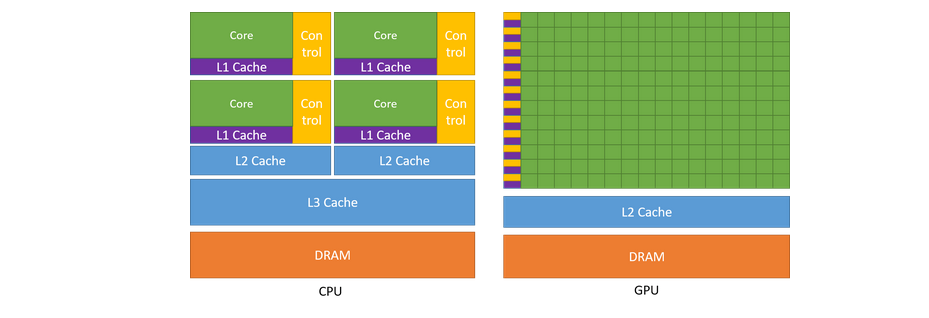
\includegraphics[scale=0.6]{img/CPUvsGPU.png}
    \caption{Architettura CPU vs architettura GPU}
\end{figure}
\noindent Questa differenza di capacità tra la GPU e la CPU esiste perché sono progettate con obiettivi diversi in mente. Mentre la CPU è progettata per eccellere nell'eseguire una sequenza di operazioni, chiamate \textit{\textbf{thread}}, il più velocemente possibile e può eseguire alcune decine di questi thread in parallelo, la GPU è progettata per eccellere nell'eseguirne migliaia in parallelo.
\noindent In generale, un'applicazione ha un mix di parti parallele e parti sequenziali, quindi i sistemi sono progettati con un mix di GPU e CPU per massimizzare le prestazioni complessive. Le applicazioni con un elevato grado di parallelismo possono sfruttare la natura massicciamente parallela della GPU per ottenere prestazioni più elevate rispetto alla CPU\cite{Nvidia-architecture}.

\section{Il ruolo di NVIDIA}
\noindent Nel 1999 NVIDIA inventa l'unità di elaborazione grafica o \textit{\textbf{GPU (Graphics Processing Unit)}}, un'idea che rivoluzionerà l'intero settore. Il lancio di GeForce 256 la descrive come prima GPU del mondo, coniando un termine che NVIDIA definisce come \emph{"un processore a chip singolo con motori integrati di trasformazione, illuminazione, creazione/clipping di triangoli e rendering in grado di elaborare un minimo di 10 milioni di poligoni al secondo"}. Le attuali GPU elaborano oltre 7 miliardi di poligoni al secondo\cite{Nvidia-story}. 
Nel corso degli anni, NVIDIA si è affermata come azienda leader nel settore, sviluppando architetture per le GPU via via più complesse e performanti. Oggi NVIDIA opera principalmente nel campo della \textit{\textbf{computer vision}} \footnote{Un campo dell'intelligenza artificiale (IA) che permette ai computer e ai sistemi di ricavare informazioni significative da immagini digitali, video e altri input visivi - e intraprendere azioni o formulare delle segnalazioni sulla base di tali informazioni.}, come ad esempio l'addestramento di veicoli per la guida autonoma.

\section{Nvidia CUDA (Compute Unified Device Architecture)}
\noindent Nel 2006 NVIDIA crea \textit{\textbf{CUDA (Compute Unified Device Architecture)}}\cite{Nvidia-story}, un'architettura sviluppata con lo scopo di utilizzare le proprie GPU dalla serie GeForce 8 in poi per eseguire eaborazioni che non siano quelle tradizionalmente legate all'ambito della computer grafica.
In questo modo, le GPU diventano totalmente programmabili e viene aggiunto il supporto a linguaggi di programmazione ad alto livello come ad esempio C e C++. Grazie all'ambiente di sviluppo CUDA è possibile utilizzare specifiche API per programmare le GPU. Ovviamente, ci sono delle specifiche API per ogni linguaggio supportato da CUDA.
\begin{figure}[h!]
    \centering
    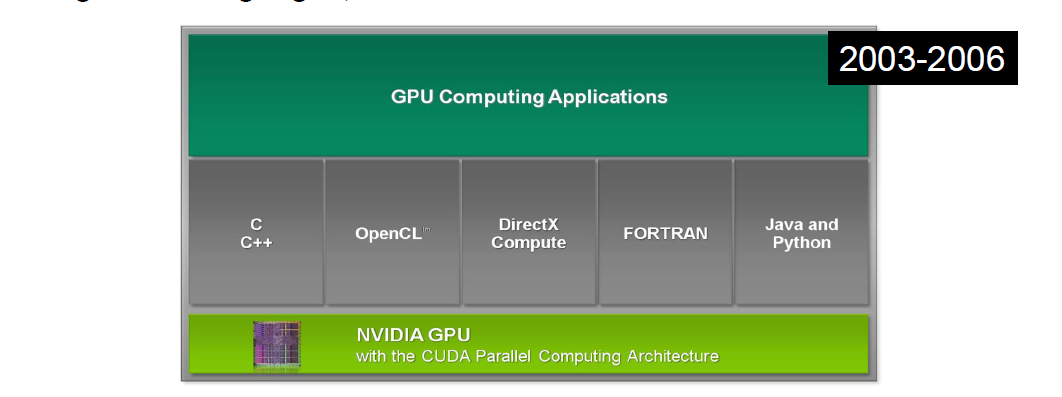
\includegraphics[scale=0.6]{img/cuda_supported_programming_languages.png}
    \caption{Alcuni dei linguaggi supportati dall'ambiente di sviluppo CUDA.}
\end{figure}

\subsection{Modello di programmazione CUDA}
\noindent Il modello di programmazione CUDA considera CPU e GPU come due macchine distinte, denominate \textit{\textbf{host}} e \textit{\textbf{device}}. Un'applicazione CUDA combina parti sequenziali (eseguite dall'host) e parti parallele (eseguite dal device). La parte di codice che lavora in parallelo è chiamata \textit{\textbf{kernel}}. L'host invoca i kernel configurando il device per l'esecuzione in parallelo, passandogli alcuni parametri. Il device può eseguire solo un kernel alla volta.

\subsubsection{Thread, block e grid}
\noindent L'unità base del parallelismo in CUDA è chiamata \textit{\textbf{thread}}: più thread eseguiti sul device eseguono lo stesso flusso di istruzioni su dati differenti, creando quello che NVIDIA ha ribattezzato come paradigma \textit{\textbf{SIMT (Single Instruction Multiple Threads}}, simile al paradigma \textit{\textbf{SIMD (Single Instruction Multiple Data)}} della \textit{\textbf{tassonomia di Flynn}}\footnote{La tassonomia di Flynn è un sistema di classificazione delle architetture dei calcolatori che classifica i sistemi di calcolo a seconda della molteplicità del flusso di istruzioni e del flusso dei dati che possono gestire}.
I thread sono raggruppati in blocchi (\textit{\textbf{blocks}}), questi blocchi vengono eseguiti sullo stesso \textit{\textbf{Streaming Multiprocessor (SM)}} e condividono una memoria condivisa che d'ora in avanti chiameremo \textit{\textbf{shared memory}}.
I blocchi sono raggruppati in una griglia (\textit{\textbf{grid}}), tutti i blocchi del device condividono una \textit{\textbf{global memory}} (la memoria della GPU). Nella Figura \ref{fig:kernel_configuration} possiamo osservare una possibile configurazione di thread e blocchi in una griglia.
\begin{figure}[h!]
    \centering
    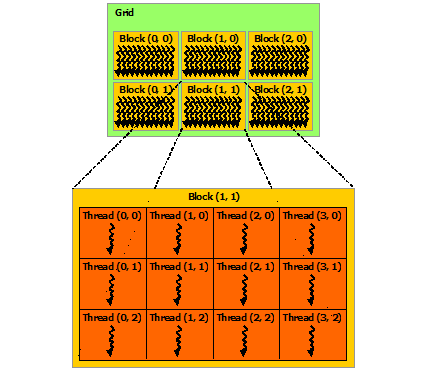
\includegraphics[scale=0.5]{img/threads_blocks_grid.png}
    \caption{Una possibile configurazione di un kernel CUDA. Una griglia 2D con $2 \times 3$ blocchi con $3 \times 4$ thread per ogni blocco.}
    \label{fig:kernel_configuration}
\end{figure}

\subsubsection{Struttura base di un'applicazione CUDA}
\noindent La struttura base di un'applicazione può essere riassunta nel seguente modo:
\begin{itemize}
    \item Prima di chiamare il kernel, l'host trasferisce i dati da elaborare sulla GPU;
    \item L'host chiama il kernel, passandogli gli argomenti appropiati di modo da permetterne la sua esecuzione;
    \item Dopo che i dati sono stati elaborati, vengono riportati sull'host dalla memoria del device.
\end{itemize}
\begin{figure}[h!]
    \centering
    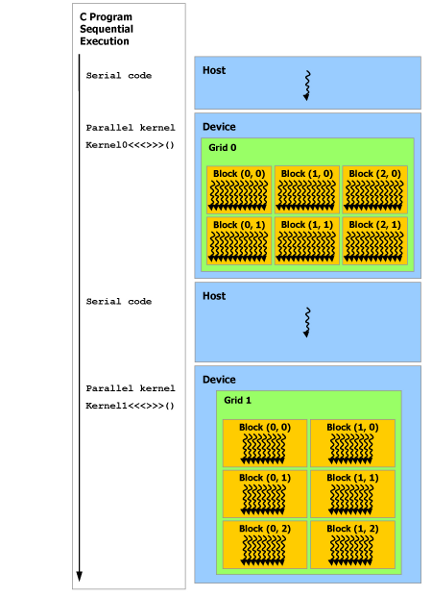
\includegraphics[scale=0.56]{img/heterogeneous-programming.png}
    \caption{Struttura base di un'applicazione cuda che evidenzia le parti sequenziali e quelle parallele.}
    \label{fig:hetero_programming}
\end{figure}

\subsection{Organizzazione della memoria}
\noindent La memoria del dispositivo è suddivisa in diverse tipologie distinguibili dalla latenza nel tempo di accesso e da quale unità è accessibile:
\begin{itemize}
    \item \textit{\textbf{Constant memory}}: area di sola lettura, per la lettura accelerata da parte di tutti i thread.
    \item \textit{\textbf{Texture memory}}: area di sola lettura, ottimizzata per la lettura e accessibile da tutti i thread.
    \item \textit{\textbf{Global memory}}: area di lettura/scrittura, esterna ai multiprocessori e condivisa tra i thread. In questo spazio, controllato dall'host, si trovano le variabili trasferite dall'host al dispositivo e viceversa. Il tempo di accesso a questa memoria è molto elevato, ma poiché essa costituisce l'interfaccia immediata con la memoria RAM della CPU, i dati devono passare per forza dalla global memory.
\end{itemize}
\begin{figure}[h!]
    \centering
    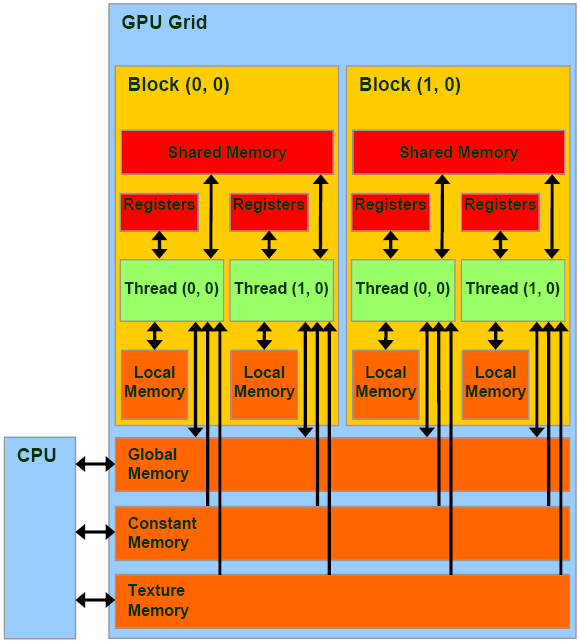
\includegraphics[scale=0.4]{img/CUDA-memory-model.png}
    \caption{Organizzazione della memoria nell'architettura CUDA.}
    \label{fig:cuda_memory_model}
\end{figure}

\subsection{Shared memory e coalescenza}
\noindent Alla classificazione della memoria della sezione precedente che si concentra sulle memorie esterne ai blocchi, possiamo aggiungere un'altra classificazione, quella delle memorie che troviamo all'interno di ciascun blocco (come riferimento si tenga presente la Figura \ref{fig:cuda_memory_model}):
\begin{itemize}
    \item \textit{\textbf{Register memory}}: memoria a bassa latenza \footnote{La latenza rappresenta i cicli di clock della memoria necessari a reperire un dato in essa memorizzato. }, privata per ogni singolo processore e accessibile da un solo thread.
    \item \textit{\textbf{Local memory}}: spazio privato per ogni singolo thread in cui sono memorizzate le variabili locali.
    \item \textit{\textbf{Shared memory}}: area di accesso a bassa latenza condivisa tra tutti i thread dello stesso blocco.
\end{itemize}
\noindent La chiave per ottenere prestazioni soddisfacenti è minimizzare gli accessi alla global memory sfruttando il più possibile la shared memory. La memoria condivisa può essere utilizzata sia come spazio privato che come spazio condiviso per la comunicazione tra i thread dello stesso blocco. Sfruttando questa capacità, i thread di uno stesso blocco possono collaborare per caricare dalla global memory alla shared memory i dati che devono essere elaborati. Successivamente provvederanno ad elaborare i dati sfruttando la minor latenza offerta dalla shared memory. Dunque i passi che ciascun thread deve eseguire sono:
\begin{itemize}
    \item caricare i dati dalla global memory alla shared memory;
    \item sincronizzare i thread di un blocco
    \item elaborare i dati nella shared memory
    \item sincronizzare nuovamente i thread per assicurarsi che tutti i thread abbiano eseguito i calcoli
    \item trasferire i dati dalla shared alla global memory
\end{itemize}
Per ottenere accessi alla memoria più veloci, i 16 KB destinati alla shared memory e condivisi tra tutti gli streaming multiprocessor, sono divisi in 16 banchi ciascuno da 1 KB, uno per ogni processore.
Come è facile intuire, per sfruttare questa memoria sono necessarie modifiche sostanziali al codice e una completa riprogettazione degli algoritmi. Tuttavia il lavoro viene ripagato da performance nettamente migliori rispetto all'algoritmo che non fa uso della shared memory. \\
I trasferimenti di dati da e verso la memoria sono governati dalla \textit{\textbf{coalescenza}}. Si indica con questo termine una serie di restrizioni che consentono di unire più accessi alla memoria in un'unica transazione. Gli accessi al kernel sono chiamati coalescenti se i thread con identificatori\footnote{Ogni CUDA thread ha un proprio identificatore (id) che lo identifica nel blocco.} consecutivi accedono a posizioni di memoria contigue utilizzando la stessa istruzione. Ciò deriva da una speciale configurazione di thread che possono essere raggruppati in \textit{\textbf{warp}}, gruppi di 32 thread che eseguono tutti la stessa istruzione.
\begin{figure}[h!]
    \centering
    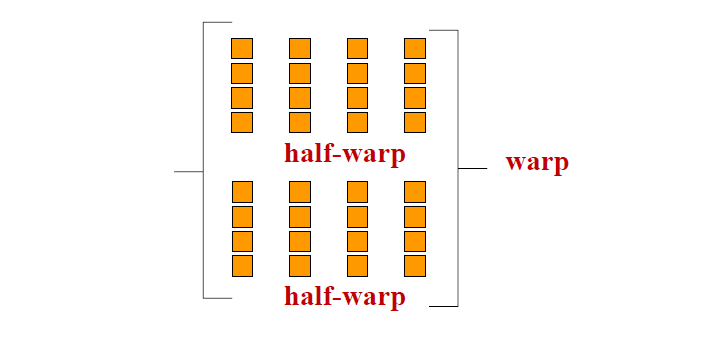
\includegraphics[scale=0.8]{img/cuda_warp.png}
    \caption{Un warp di thread (32 thread) diviso un due warp da 16 thread ciascuno.}
    \label{fig:cuda_warp}
\end{figure}

\section{API di CUDA per il linguaggio C}
\noindent CUDA mette a disposizione delle API per il linguaggio C, che rendono semplice e intuitivo l'allocazione di dati sul device, il trasferimento di dati da host a device e viceversa, la creazione e la configurazione di kernel e molto altro. Nelle sezioni successive verrà analizzata la struttura base di programma CUDA, concentrandosi in particolar modo su quali sono le funzioni di libreria che vengono più spesso utilizzate e come i dati devono essere allocati. Inoltre viene proposto un esempio banale di kernel che effettua la somma puntuale di due vettori di interi.

\subsection{Struttura base di un programma CUDA}
\noindent Un programma in \textit{\textbf{CUDA C}} deve necessariamente includere l'header \texttt{<cuda.h>}, ove sono contenute tutte le funzioni di libreria necessarie al programma. La struttura base di un programma può essere riassunta nei seguenti passi:
\begin{itemize}
    \item dichiarazione delle variabili dell'host
    \item dichiarazione delle variabili del device
    \item allocazione dei dati dell'host con \texttt{malloc}
    \item allocazione dei dati del device con \texttt{cudaMalloc}
    \item inizializzazione dei dati dell'host
    \item copia dei dati da host a device con la funzione \texttt{cudaMemcpy}
    \item invocazione kernel: configurazione dei parametri
    \item copia dei risultati da device a host con la funzione \texttt{cudaMemcpy}
    \item deallocazione dei dati dell'host con la funzione \texttt{freee}
    \item deallocazione dei dati del device con la funzione \texttt{cudaFree}
\end{itemize}
Tutte le operazioni in CUDA sono fatte per mezzo di puntatori. Vettori e matrici devono essere allocati dinamicamente e in particolare, le matrici devono essere allocate come se fossero dei vettori. Esempio: se la matrice $A$ ha dimensioni $M \times N$, deve essere allocato un array di dimensioni $M \times N$.

\lstinputlisting[language=C, caption=Esempio allocazione matrice dell'host con CUDA]{code/cuda_allocation.c}

\noindent Di conseguenza, per accedere ad un elemento della matrice \texttt{a} non si usa la seguente sintassi \texttt{a[i][j]} ma la sintassi per accedere ad un elemento in posizione \texttt{i,j} è \texttt{a[i * N + j]}, dove $N$ è il numero di colonne della matrice è costituisce la cosiddetta \textit{\textbf{leading dimension}}\footnote{La leading dimension per una matrice è un incremento utilizzato per trovare il punto iniziale per gli elementi della matrice in ogni colonna successiva della matrice.\cite{leading-dimension}}. \\
\noindent Di seguito si riporta un banale programma cuda che non fa altro che copiare un array da host a device e poi di nuovo da device ad host.
\vspace{0.5cm}

\noindent Librerie da includere:
\lstinputlisting[language=C, firstline=1, lastline=3, caption=Librerie richieste dall'ambiente CUDA]{code/first_cuda.c}

\newpage
\noindent Funzione main del programma:
\lstinputlisting[language=C, firstline=9, lastline=62, caption=Inizializzazione e copia di una matrice host-device e device-host]{code/first_cuda.c}

\noindent Funzioni helper:
\lstinputlisting[language=C, firstline=64, lastline=85, caption=Funzioni utilizzate nel precedente listato]{code/first_cuda.c}

\subsection{Funzioni di libreria più utilizzate}
\noindent Dopo aver illustrato un semplice esempio di programma CUDA C, analizziamo un po' più nel dettaglio quali sono le funzioni di libreria più utilizzate.

\subsubsection{Allocazione della memoria su GPU}
\begin{lstlisting}[language=C]
    cudaError_t cudaMalloc(void **devPtr, size_t size);
\end{lstlisting}
\begin{itemize}
    \item \texttt{devPtr} - puntatore all'area di memoria da allocare sul device
    \item \texttt{size} - la dimensione in byte dell'area da allocare
\end{itemize}

\subsubsection{Deallocazione della memoria su GPU}
\begin{lstlisting}[language=C]
    cudaError_t cudaFree(void *devPtr);
\end{lstlisting}
\begin{itemize}
    \item \texttt{devPtr} - puntatore all'area di memoria da deallocare sul device
\end{itemize}

\subsubsection{Scambio di dati tra CPU e GPU}
\begin{lstlisting}[language=C]
    cudaError_t cudaMemcpy(
        void *dest, 
        void *src, 
        size_t nBytes, 
        enum cudaMemcpyKind
    );
\end{lstlisting}
\begin{itemize}
    \item \texttt{dest} - puntatore all'area di memoria in cui copiare
    \item \texttt{src} - puntatore all'area di memoria da cui copiare
    \item \texttt{nBytes} - la dimensione in byte dell'area di memoria da copiare
    \item \texttt{cudaMemcpyKind} - indica la direzione della copia. È una variabile che può assumere i seguenti valori:
    \begin{itemize}
        \item \texttt{cudaMemcpyHostToHost} copia i dati da host a host
        \item \texttt{cudaMemcpyHostToDevice} copia i dati da host a device
        \item \texttt{cudaMemcpyDeviceToHost} copia i dati da device a host
        \item \texttt{cudaMemcpyDeviceToDevice} copia i dati da device a device
    \end{itemize}
\end{itemize}

\subsection{Creazione e configurazione di un kernel}
\noindent Di seguito si riporta l'esempio di un kernel che effettua la somma puntuale di due vettori di \texttt{float} e la memorizza in un terzo vettore. Per semplicità si omettono tutte le parti relative all'allocazione e alla deallocazione di variabili.

\vspace{0.5cm}
\lstinputlisting[language=C,  caption=Configurazione di un kernel per la somma di due vettori.]{code/kernel_example.c} \label{list: ex01}
\vspace{0.5cm}

\noindent Le funzioni CUDA hanno lo stesso prototipo delle solite funzioni C precedute da uno di questi qualificatori:
\begin{itemize}
    \item \texttt{\_\_global\_\_} : per le funzioni chiamate dall'host ed eseguite sul device (i kernel)
    \item \texttt{\_\_device\_\_} : per le funzioni chiamate dal device ed eseguite sul device
    \item \texttt{\_\_host\_\_}: (opzionale) per le funzioni eseguite dalla CPU
\end{itemize}

\noindent Il tipo di dato \texttt{dim3} è un tipo predefinito di CUDA che rappresenta un vettore di tre interi; questi tre campi sono accessibili con le notazioni \texttt{.x}, \texttt{.y}, \texttt{.z} e servono per indicare il numero dei fili o il numero dei blocchi in una particolare direzione; gli eventuali campi non dichiarati vengono automaticamente impostati a 1.
\begin{itemize}
    \item \texttt{nBlocks} è il numero di blocchi della griglia, può essere 1D o 2D
    \item \texttt{nThreadsPerBlock} è il numero di thread per un singolo blocco (1D, 2D o 3D)
\end{itemize}

\subsubsection{Esempio}
\noindent Supponiamo di usare $N = 12$. Fissando il numero di blocchi a 3 come nell'esempio \ref{list: ex01}, il numero di thread per ciascun blocco sarà pari a 4, poiché $12 / 3 = 4$. Nel caso N non fosse stato esattamente divisibile per il numero di blocchi, al numero di thread sarebbe stato aggiunto un 1 e alcuni thread non avrebbero partecipato al calcolo della somma.

\begin{figure}[h!]
    \centering
    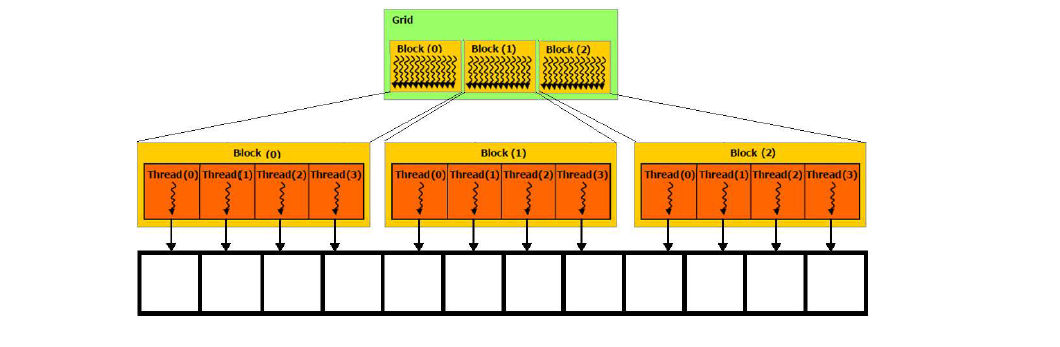
\includegraphics[scale=0.6]{img/kconf.png}
    \caption{Configurazione del kernel CUDA \texttt{VecAdd} con N = 12 e numero di blocchi pari a 3.}
\end{figure}
\def\baselinestretch{1}
\chapter{Approccio parallelo e implementazione in ambiente GPU} \label{cap:approccio-parallelo}
\chaptermark{Approccio parallelo su GPU}
\def\baselinestretch{1.66}

%%%%%%%%%%%%%%%%%%%%%%%%%%%%%%%%%%%%%%%%%%%%%%%%%%%%%%%%%%%%%%%
%                   Approccio parallelo
%%%%%%%%%%%%%%%%%%%%%%%%%%%%%%%%%%%%%%%%%%%%%%%%%%%%%%%%%%%%%%%
\section{Approccio parallelo} \label{sec:approccio-parallelo}
\noindent Nel capitolo \ref{cap:modello-numerico} sezione \ref{sec:approccio-sequenziale} è stato analizzato l'algoritmo sequenziale per la risoluzione della PDE (Partial Differential Equation) proposta in questo lavoro. A causa dell'elevato tempo di calcolo richiesto dalla procedura sequenziale per trovare la soluzione dell'equazione (\ref{eq:peer-methods-1}) all'aumentare di $N$ (si rimanda alla sezione \ref{sec:sequential_test} per approfondimenti), si è scelto di parallelizzare il modulo relativo al calcolo di tale equazione. Prima di passare direttamente alla presentazione del codice parallelo e della strategia di parallelizzazione adottata, vengono illustrare le operazioni preliminari svolte per la stesura dell'algoritmo parallelo.

%--------------------------------------------------------------
%                   Operazioni preliminari
%--------------------------------------------------------------
\subsection{Operazioni preliminari} \label{subsec:approccio-parallelo-operazioni-preliminari}
\noindent Il primo passo effettuato nel processo di parallelizzazione dell'algoritmo sequenziale \ref{alg:peerMethodsSequential} è stato quello di ottimizzare il modo in cui è memorizzata la matrice $L$ definita in (\ref{eq:matrix-L}). Tale matrice è una matrice tridiagonale a blocchi, che presenta un gran numero di valori nulli che non influiscono in alcun modo nelle operazioni in cui è coinvolta la matrice, rendendo quindi inutile salvarli in memoria. L'approccio che si utilizza in questi casi (e che è stato utilizzato) è quello di memorizzare la matrice $L$ in formato \textit{\textbf{CSR (Compressed Sparse Row)}}. Il formato CSR è pensato per memorizzare una matrice con un gran numero di zeri in maniera compatta, eliminando tutti i valori nulli e memorizzando solo i valori non nulli (chiamati non-zero values, talvolta abbreviato in nnz). Il formato prevede di dichiarare tre array che chiameremo rispettivamente \texttt{row\_ptrs}, \texttt{col\_ids} e \texttt{vals}. L'array \texttt{row\_ptr} fornisce la somma cumulativa degli elementi diversi da zero in ogni riga e quindi ha dimensione $m + 1$ per una matrice sparsa $m \times n$. L'array \texttt{col\_ids} fornisce l'indice della colonna e l'array \texttt{vals} fornisce i valori per ciascuno degli elementi diversi da zero. Pertanto, il formato CSR richiede $2 \times nnz + m + 1$ di spazio di allocazione. Se il numero di nnz è particolarmente ridotto, come nel caso della matrice $L$, si ha una diminuzione sia dello spazio di allocazione e sia nel numero di operazioni che vengono svolte.

\noindent Di seguito si riporta un esempio del formato CSR applicato a una matrice tridiagonale a blocchi $A$ di $4 \times 4$ elementi e con gli indici che partono da 0.

\begin{equation*}
    A = \begin{bmatrix} 
	-2 & 1 & 0 & 1\\
	1 & -2 & 1 & 0\\
	0 & 1 & -2 & 1\\
    1 & 0 & 1 & -2
	\end{bmatrix}
	\quad
\end{equation*}

\begin{equation*}
    \texttt{row\_ptrs} \quad [0 \quad 3 \quad 6 \quad 9 \quad 12] \\
\end{equation*}
\begin{equation*}
    \texttt{col\_idxs} \quad [0 \quad 1 \quad 3 \quad 0 \quad 1 \quad 2 \quad 1 \quad 2 \quad 3 \quad 0 \quad 2 \quad 3] \\
\end{equation*}
\begin{equation*}
    \texttt{vals} \quad [-2 \quad 1 \quad 1 \quad  1 \quad -2 \quad 1 \quad 1 \quad -2 \quad 1 \quad 1 \quad 1 \quad -2] \\
\end{equation*}

%--------------------------------------------------------------
%                   Algoritmo parallelo
%--------------------------------------------------------------
\section{Algoritmo parallelo} \label{subsec:approccio-parallelo-algoritmo-parallelo}
\noindent Lo pseudo-codice parallelo \ref{alg:peerMethodsParallel} evidenzia i passi principali della procedura numerica in un ambiente GPU. I dettagli e le operazioni principali sono elencati nei seguenti passaggi:

\newpage

\begin{breakablealgorithm}
    \caption{Algoritmo parallelo peer methods}\label{alg:peerMethodsParallel}
    \vspace{0.5cm}
    \textbf{Input} $s,x_0,X,N, t_0, T,M, y_0,N, L, a,B_1,B_2,H, F, S, d, D, \Delta t$. \quad
    \textbf{Output} $Y$
    \vspace{0.2cm}
    \begin{algorithmic}[1]
        \Statex \textbf{// Initialization}
        \State $t\_span = [t_0, T]$
        \State time discretization $t_n(n = 0, \ldots, N)$
        \State $N = (t\_span[2]-t\_span[1])/\Delta t$
        \State $x\_span = [x_0, X]$
        \State space discretization $x_m(m = 0, \ldots, M - 1)$
        \State $\Delta x = (x\_span[2]-x\_span[1])/(M - 1)$
        \Statex \textbf{// Sequential spatial discretization}
        \State building of $L_{Diff}$ and $L$ as in \eqref{eq:matrix-Ldiff}, \eqref{eq:matrix-L}
        \State convert $L$ from dense to sparse matrix in CSR format
        \Statex \textbf{// Parallel time discretization using peer method}
        \State $s = 2$
        \Statex // GPU computation start
        \State \texttt{transfer} Input data from Host-To-Device
        \Statex // Initialization with time step $n = 0$
        \State \texttt{parallel computing} of $Y_{0,1}$ and $Y_{0,2}$ using Runge-Kutta 4th order method
        \State \texttt{parallel evaluation} of $\mathcal{F}((Y_{0,1}))$ and $\mathcal{F}((Y_{0,2}))$ as in \eqref{eq:FYnm1-equation}
        \Statex // Main loop: loop on time steps
        \For {$n = 1 \ldots N$} 
        \State \texttt{parallel computing} $Y_{n,1}$ and $Y_{n,2}$ as in \eqref{eq:extended-peer-methods}
        \State \texttt{parallel evaluation} of $\mathcal{F}((Y_{n,1}))$ and $\mathcal{F}((Y_{n,2}))$ as in \eqref{eq:FYnm1-equation}
        \EndFor
        \State \texttt{transfer} Output data from Device-To-Host
        \Statex // GPU computation end
    \end{algorithmic}
\end{breakablealgorithm}
\vspace{0.2cm}
%--------------------------------------------------------------
%                Spiegazione pseudocodice
%--------------------------------------------------------------
\begin{itemize}
    \item \texttt{Righe 2-7}: l'algoritmo inizializza i parametri necessari per la discretizzazione del tempo e dello spazio così come nella controparte sequenziale \ref{alg:peerMethodsSequential}.
    
    \item \texttt{Righe 9-10}: dopo aver definito la matrice $L$ così come è stato fatto nell'algoritmo \ref{alg:peerMethodsSequential}, la si converte in formato CSR (Compressed Sparse Row). L'algoritmo per la definizione della matrice $L$ in formato CSR è il seguente:
    \begin{breakablealgorithm}
        \caption{Definizione matrice in formato CSR}\label{alg:CSRAlg}
        \vspace{0.5cm}
        \textbf{Input} $A, nrows, ncols, nnz$ \\
        \textbf{Output} $row\_ptrs, col\_idxs, values$
        \vspace{0.5cm}
        \begin{algorithmic}[1]
            \State \texttt{allocate} $row\_ptrs[1\ldots nrwos + 1]$
            \State \texttt{allocate} $col\_idxs[1 \ldots nnz]$
            \State \texttt{allocate} $values[1 \ldots nnz]$
            \State $cumulative\_sum = 0$
            \For {$i = 1 \ldots nrows$}
                \State $row\_ptrs[i] = cumulative\_sum$
                \For {$j = 1 \ldots ncols$}
                    \State $col\_idxs[cumulative\_sum] = j$
                    \State $values[cumulative\_sum] = A[i, j]$
                    \State $cumulative\_sum = cumulative\_sum + 1$
                \EndFor
            \EndFor
            \State $row\_ptrs[nrows] = cumulative\_sum$
        \end{algorithmic}
    \end{breakablealgorithm}

    \begin{itemize}
        \item \texttt{Righe 1-4}: inizializzazione e allocazione delle strutture dati ossia $row\_ptrs$, $col\_idxs$, $values$.
        \item \texttt{Righe 5-12}: viene costruita la matrice sparsa. Il ciclo for più esterno costruire l'array $row\_ptrs$, quello più interno $col\_idxs$ e $values$ salvando rispettivamente gli indici di colonna e i valori diversi da zero all'interno di queste due strutture dati.
    \end{itemize}
    
    \item \texttt{Righe 16-17}: si procede con il calcolo di $Y_{0, i}$ dove $i = 1 \ldots s$, utilizzando il metodo Runge-Kutta del quarto ordine, che è stato parallelizzato distribuendo le operazioni di algebra lineare su un opportuno numero di thread. Anche la valutazione della funzione $\mathcal{F}$ è stata parallelizzata, distribuendo le operazioni tra un opportuno numero di thread.
    \newpage
    \begin{breakablealgorithm}
        \caption{Algoritmo di Runge-Kutta parallelo}\label{alg:RK4Alg}
        \vspace{0.5cm}
        \textbf{Input} $h, t_0, y_0$ \\
        \textbf{Output} $y$
        \vspace{0.5cm}
        \begin{algorithmic}[1]
            \Statex // Compute $Y_1$
            \State $Y_1 = y_0$
            \Statex // Compute $Y_2$
            \State \texttt{parallel evaluation} of $\mathcal{F}(Y_1)$
            \State \texttt{parallel product} $h / 2$ by $\mathcal{F}(Y_1)$
            \State $Y_2 =$ \texttt{parallel sum} $y_0 + \mathcal{F}(Y_1)$
            \Statex // Compute $Y_3$
            \State \texttt{parallel evaluation} of $\mathcal{F}(Y_2)$
            \State \texttt{parallel product} $h / 2$ by $\mathcal{F}(Y_2)$
            \State $Y_3 =$ \texttt{parallel sum} $y_0 + \mathcal{F}(Y_2)$
            \Statex // Compute $Y_4$
            \State \texttt{parallel evaluation} of $\mathcal{F}(Y_3)$
            \State \texttt{parallel product} $h$ by $\mathcal{F}(Y_3)$
            \State $Y_4 =$ \texttt{parallel sum} $y_0 + \mathcal{F}(Y_3)$
            \Statex // Make a sort of weighted arithmetic mean
            \State $y = y_0 + h \cdot (1/6 \cdot \mathcal{F}(Y_1) + 1/3 \cdot \mathcal{F}(Y_2) + 1/3 \cdot \mathcal{F}(Y_3) + 1/6 \cdot \mathcal{F}(Y_4))$
        \end{algorithmic}
    \end{breakablealgorithm}
    
    \item \texttt{Righe 20-21}: ancora una volta il loop principale non fa altro che eseguire le stesse operazioni eseguite al di fuori del loop, dato che ogni step è funzione del precedente come è stato ampiamente discusso nel capitolo \ref{cap:modello-numerico}. Si calcola in parallelo $Y_{n, i}$ dove $i = 1 \ldots s$ ed $n = 1 \ldots N$ secondo l'equazione \eqref{eq:peer-methods-1}, eseguendo parallelamente gli $s$ stage della variabile $j$. La valutazione della funzione $\mathcal{F}$ è praticamente la stessa effettuata alla riga \texttt{17}.
\end{itemize}

\noindent Nella paragrafo successivo verrà analizzata in dettaglio la strategia di parallelizzazione utilizzata per il calcolo dell'equazione (\ref{eq:peer-methods-1}) in ambiente CUDA (riga 20 dell'algoritmo parallelo \ref{alg:peerMethodsParallel}), in quanto per la sua importanza merita un approfondimento in più.

%--------------------------------------------------------------
%                   computeYGPU
%--------------------------------------------------------------
\subsection{Strategia di parallelizzazione kernel dell'equazione principale } \label{computeYGPU-par}
\noindent Per capire qual è il processo che ha portato alla parallelizzazione dell'equazione (\ref{eq:peer-methods-1}) in ambiente CUDA, la si può riscrivere in forma più compatta come segue:

\begin{equation}
    Y_{n, i} =  b_{ij}Y_{n - 1, j} + h a_{ij} f(t_{n - 1, j}, Y_{n - 1, j})
    \label{eq:parallel-peer-methods-compressed}
\end{equation}

\begin{equation*}
    \text{con } n = 2\ldots N \quad i = 1\ldots s \quad j = 1\ldots s \nonumber
\end{equation*}

\noindent Poiché $s = 2$, andiamo ad esplicitare la $j$ e otteniamo due equazioni:
\begin{gather}
    Y_{n, 1} =  b_{i1}Y_{n - 1, 1} + h a_{i1} f(t_{n - 1, 1}, Y_{n - 1, 1}) \nonumber \\ 
    Y_{n, 2} =  b_{i2}Y_{n - 1, 2} + h a_{i2} f(t_{n - 1, 2}, Y_{n - 1, 2})
    \label{eq:parallel-peer-methods-unrolled}
\end{gather}

\noindent Una volta ottenuta l'equazione in questa forma, bisogna capire come implementare i vari attori che la compongono. Sia $d$ la dimensione del problema, $Y$ può essere visto come una matrice di dimensione $s \cdot d \times N$, ove i primi $d$ valori rappresentano la soluzione $Y_{n,1}$ e i restanti $d$ valori rappresentano $Y_{n,2}$. $A$ e $B$ sono due matrici $2 \times 2$ la cui configurazione è quella in (\ref{eq:ABc-equation}) e la funzione $f$ viene calcolata seguendo l'equazione \eqref{eq:ODE-system-disc} e poiché la dimensione del problema è $d$, sarà un vettore di $d$ elementi.

\begin{figure}[ht!]
    \centering
    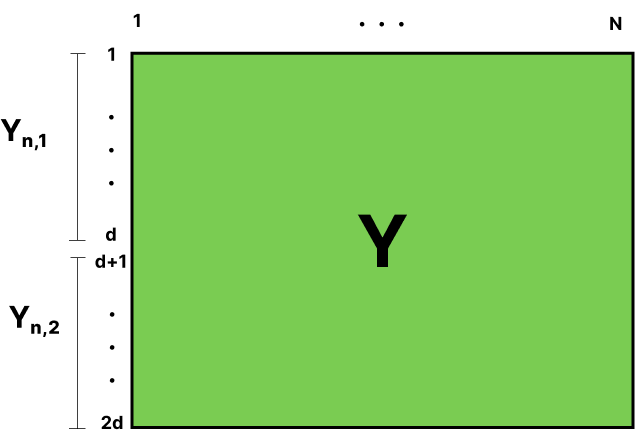
\includegraphics[scale=0.25]{img/MatrixY075x.png}
    \caption{Struttura della matrice Y.}
    \label{fig:matrixYstructure}
\end{figure}

\noindent L'implementazione della strategia di parallelizzazione consiste nel creare un kernel apposito per il calcolo di $Y_{n,1}$ e $Y_{n,2}$ per ogni $n = 2,\ldots,N$ e nello sfruttare l'architettura CUDA, che ci consente di organizzare i thread in blocchi (come spiegato nel capitolo \ref{cap:GPU}). Sia i thread che i blocchi possono essere bidimensionali, cioè è possibile scegliere una griglia di thread all'interno di una griglia di blocchi. I thread presenti nello stesso blocco godono di alcuni vantaggi, come ad esempio possono condividere alcuni registri in modo da eseguire in maniera più efficienti le operazioni assegnate. L'implementazione della strategia di parallelizzazione proposta mira a fare in modo che la griglia con cui viene lanciato il kernel sia bidimensionale, ossia ci siano fissi due blocchi lungo l'asse y e un numero di blocchi lungo l'asse delle x che può essere arbitrario. Anche il numero di thread all'interno di ciascun blocco può essere arbitrario, purché non sia in numero maggiore rispetto agli elementi della matrice $Y$ su cui bisogna operare. La distribuzione del lavoro tra i vari thread e i vari blocchi avviene dividendo la dimensione del problema $d$ per il prodotto tra il numero di thread e il numero di blocchi. Disponendo di una griglia bidimensionale di blocchi, considerando che ciascun blocco ha una coppia di identificativi chiamati rispettivamente \texttt{blockIdx.x} e \texttt{blockIdx.y}, i blocchi con \texttt{blockIdx.y} = 0 calcoleranno l'equazione (\ref{eq:parallel-peer-methods-unrolled}) per $i = 1$ e i blocchi con \texttt{blockIdx.y} = 1 calcoleranno la medesima equazione per $i = 2$ concorrentemente. Osservando la figura \ref{fig:matrixYstructure} si può notare che ciascun stage $i$ opera su porzioni differenti della matrice $Y$ e questo fa sì che non possano verificarsi race condition sugli elementi della matrice.

\begin{figure}[ht!]
    \centering
    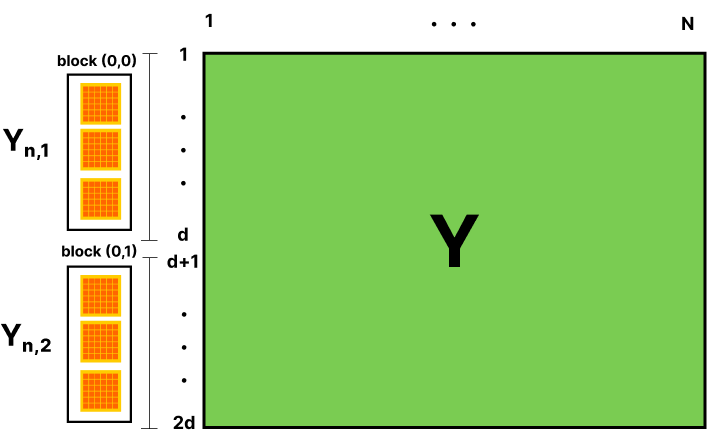
\includegraphics[scale=0.35]{img/YwBlocks.png}
    \caption{Distribuzione dei valori della matrice $Y$ fra thread e blocchi.}
    \label{fig:matrixYstructure}
\end{figure}
\def\baselinestretch{1}
\chapter{Test, risultati e conclusioni} \label{cap:test}
\def\baselinestretch{1.66}

%--------------------------------------------------------------
%                   Test parallelo
%--------------------------------------------------------------
\section{Confronto tempi GPU vs CPU} \label{sec:parallel_test}
\noindent In questa sezione andremo a confrontare i tempi dell'algoritmo sequenziale con quelli dell'algoritmo parallelo per ciascun macro modulo che è stato individuato nel problema (\ref{eq:main-equation}). Verrà mostrato quindi come l'accelerazione parallela dell'algoritmo \ref{alg:peerMethodsSequential} ha portato ad una notevole riduzione nei tempi di esecuzione sia dei vari macro moduli e sia del software nel suo complesso. Per il resto della sezione, consideriamo il problema (\ref{eq:main-equation}) con i seguenti parametri di input $A = 1.5$, $B_1 = 0.45$, $B_2 = 0.3611$, $F = 0.802$, $H = 0.802$, $S = 0.0002$, $d = 500$, $D = 0.802$, e gli intervalli di spazio e tempo pari rispettivamente a $\left[-50, 50\right]$ e $[0, 50]$. Inoltre, gli esperimenti sono stati eseguiti su un  computer con le seguenti specifiche tecniche:
\begin{itemize}
    \item 4 Intel(R) Core(TM) i7 860 CPU @2.80 GHz, 4 core, 8 thread per core, 8 GB di RAM
    \item 1 GPU NVIDIA Quadro K5000, 1536 cuda core, 4 GB GDDR5, 173 GB/s di banda
\end{itemize}

\noindent Si noti che in ciascuna tabella, moltiplicando il numero di chiamate delle funzioni per il tempo medio si ottiene il tempo totale di esecuzione della specifica funzione.

\newpage

%%%%%%%%%%%%%%%%%%%%%%%%%%%%%%%%%%%%%%%%%%%%%%%%%%%%%%%%%%%%
%                       16x12
%%%%%%%%%%%%%%%%%%%%%%%%%%%%%%%%%%%%%%%%%%%%%%%%%%%%%%%%%%%%
\subsection{Thread $\times$ block: 16 $\times$ 12}

% ooooooooooooooooooooooooooooooooooooooooooooooooooooooooooooo
%                       Old tables
% ooooooooooooooooooooooooooooooooooooooooooooooooooooooooooooo
\begin{comment}
%--------------------------------------------------------------
%                   Runge Kutta 16x12
%--------------------------------------------------------------
\begin{table}[ht!]
    \begin{center}
        \renewcommand{\arraystretch}{1.5}
        \begin{adjustbox}{width=.51\textwidth}
            \begin{tabular}{ |c|c|c|c|c| }
                \hline
                \multicolumn{1}{|c}{} & \multicolumn{1}{|c}{RungeKutta4th GPU} & \multicolumn{1}{|c|}{RungeKutta4th CPU} \\
                \hline
                N & Tempo medio(s) & Tempo medio(s) \\
                \hline 
                $1 \times 10^2$ & $4.2848 \times 10^{-5}$ & $2.3065 \times 10^{-3}$ \\
                \hline 
                $1 \times 10^3$ & $4.6192 \times 10^{-5}$ & $3.1820 \times 10^{-3}$ \\
                \hline 
                $1 \times 10^4$ & $4.6559 \times 10^{-5}$ & $2.9975 \times 10^{-3}$ \\
                \hline 
                $1 \times 10^5$ & $4.6160 \times 10^{-5}$ & $3.2775 \times 10^{-3}$ \\ 
                \hline 
                $1 \times 10^6$ & $4.6336 \times 10^{-5}$ & - \\
                \hline 
            \end{tabular}
        \end{adjustbox}
    \end{center}
    \caption{Confronto tempi di esecuzione modulo RungeKutta4th su GPU vs CPU per la configurazione 16 thread e 12 blocchi}
    \label{tab:rk4_kernel_table_16x12}
\end{table}

%--------------------------------------------------------------
%                       Sherratt 16x12
%--------------------------------------------------------------
\begin{table}[ht!]
    \begin{center}
        \renewcommand{\arraystretch}{1.5}
        \begin{adjustbox}{width=.65\textwidth}
            \begin{tabular}{ |c|c|c|c|c| }
                \hline
                \multicolumn{1}{|c}{} & \multicolumn{2}{|c}{Sherratt GPU} & \multicolumn{2}{|c|}{Sherratt CPU} \\
                \hline
                N & Chiamate & Tempo medio(s) & Chiamate & Tempo medio(s) \\
                \hline 
                $1 \times 10^2$ & $2 \times 10^{2}$ & $6.4120 \times 10^{-6}$  & $2 \times 10^{2}$ & $6.9000 \times 10^{-3}$ \\
                \hline 
                $1 \times 10^3$ & $3 \times 10^{3}$ & $6.4160 \times 10^{-6}$  & $3 \times 10^{3}$ & $6.5293 \times 10^{-3}$ \\
                \hline 
                $1 \times 10^4$ & $2 \times 10^{4}$ & $6.4270 \times 10^{-6}$  & $2 \times 10^{4}$ & $6.5230 \times 10^{-3}$ \\
                \hline 
                $1 \times 10^5$ & $2 \times 10^{5}$ & $6.4280 \times 10^{-6}$  & $2 \times 10^{5}$ & $2.7116 \times 10^{-4}$ \\
                \hline 
                $1 \times 10^6$ & $3 \times 10^{6}$ & $6.4290 \times 10^{-6}$  & - & - \\ 
                \hline 
            \end{tabular}
        \end{adjustbox}
    \end{center}
    \caption{Confronto tempi di esecuzione modulo Sherratt su GPU vs CPU per la configurazione 16 thread e 12 blocchi}
    \label{tab:sherratt_kernel_table_16x12}
\end{table}

%--------------------------------------------------------------
%                   computeY 16x12
%--------------------------------------------------------------
\begin{table}[ht!]
    \begin{center}
        \renewcommand{\arraystretch}{1.5}
        \begin{adjustbox}{width=.65\textwidth}
            \begin{tabular}{ |c|c|c|c|c| }
                \hline
                \multicolumn{1}{|c}{} & \multicolumn{2}{|c}{computeY GPU} & \multicolumn{2}{|c|}{computeY CPU} \\
                \hline
                N & Chiamate & Tempo medio(s) & Chiamate & Tempo medio(s) \\
                \hline 
                $1 \times 10^2$ & $1 \times 10^{2}$ & $4.1140 \times 10^{-6}$ & $1 \times 10^{2}$ & $2.8554 \times 10^{-4}$ \\
                \hline 
                $1 \times 10^3$ & $1 \times 10^{3}$ & $4.1730 \times 10^{-6}$ & $1 \times 10^{3}$ & $2.6946 \times 10^{-4}$ \\
                \hline 
                $1 \times 10^4$ & $1 \times 10^{4}$ & $4.1150 \times 10^{-6}$ & $1 \times 10^{4}$ & $2.6829 \times 10^{-4}$ \\
                \hline 
                $1 \times 10^5$ & $1 \times 10^{5}$ & $4.0730 \times 10^{-6}$ & $1 \times 10^{5}$ & $1.2223 \times 10^{-5}$ \\
                \hline 
                $1 \times 10^6$ & $1 \times 10^{6}$ & $4.0800 \times 10^{-6}$ & - & - \\ 
                \hline 
            \end{tabular}
        \end{adjustbox}
    \end{center}
    \caption{Confronto tempi di esecuzione modulo computeY su GPU vs CPU per la configurazione 16 thread e 12 blocchi}
    \label{tab:computeY_kernel_table_16x12}
\end{table}

\vspace{3cm}

%--------------------------------------------------------------
%                    Total time 16x12
%--------------------------------------------------------------
\begin{table}[ht!]
    \begin{center}
        \renewcommand{\arraystretch}{1.5}
        \begin{adjustbox}{width=.45\textwidth}
            \begin{tabular}{ |c|c|c| }
                \hline
                \multicolumn{1}{|c}{} & \multicolumn{2}{|c|}{Tempo totale modulo (s)} \\
                  \hline
                  N & GPU & CPU \\
                  \hline
                  $1 \times 10^2$ & $1.333 \times 10^{-2}$ & $1.4151$ \\
                  \hline 
                  $1 \times 10^3$ & $1.4267 \times 10^{-1}$ & $2.1347 \times 10$ \\
                  \hline 
                  $1 \times 10^4$ & $9.79015 \times 10^{-1}$ & $1.7056 \times 10^{2}$ \\
                  \hline 
                  $1 \times 10^5$ & $8.0828$ & $5.7871 \times 10$ \\
                  \hline 
                  $1 \times 10^6$ & $1.2801 \times 10^{2}$ & - \\
                  \hline 
            \end{tabular}
        \end{adjustbox}
    \end{center}
    \caption{Tempo di esecuzione GPU vs CPU per 16 thread e 12 blocchi}
    \label{tab:time_table_16x12}
\end{table}
\end{comment}


%--------------------------------------------------------------
%                   Runge Kutta 16x12
%--------------------------------------------------------------
\begin{table}[ht!]
    \begin{center}
        \renewcommand{\arraystretch}{1.5}
        \begin{adjustbox}{width=.51\textwidth}
            \begin{tabular}{ |c|c|c|c|c| }
                \hline
                \multicolumn{1}{|c}{} & \multicolumn{1}{|c}{RungeKutta4th GPU} & \multicolumn{1}{|c|}{RungeKutta4th CPU} \\
                \hline
                N & Tempo medio(s) & Tempo medio(s) \\
                \hline 
                $1 \times 10^5$ & $4.6160 \times 10^{-5}$ & $3.2775 \times 10^{-3}$ \\
                \hline 
                $2 \times 10^5$ & $4.6208 \times 10^{-5}$ & $3.0250 \times 10^{-3}$ \\
                \hline 
                $4 \times 10^5$ & $4.6000 \times 10^{-5}$ & $3.1805 \times 10^{-3}$ \\
                \hline 
                $8 \times 10^5$ & $4.6400 \times 10^{-5}$ & $2.8115 \times 10^{-3}$ \\ 
                \hline 
                $1 \times 10^6$ & $4.6336 \times 10^{-5}$ & - \\
                \hline 
                $3 \times 10^6$ & - & - \\
                \hline
            \end{tabular}
        \end{adjustbox}
    \end{center}
    \caption{Confronto tempi di esecuzione modulo RungeKutta4th su GPU vs CPU per la configurazione 16 thread e 12 blocchi}
    \label{tab:rk4_kernel_table_16x12}
\end{table}

%--------------------------------------------------------------
%                       Sherratt 16x12
%--------------------------------------------------------------
\begin{table}[ht!]
    \begin{center}
        \renewcommand{\arraystretch}{1.5}
        \begin{adjustbox}{width=.65\textwidth}
            \begin{tabular}{ |c|c|c|c|c| }
                \hline
                \multicolumn{1}{|c}{} & \multicolumn{2}{|c}{Sherratt GPU} & \multicolumn{2}{|c|}{Sherratt CPU} \\
                \hline
                N & Chiamate & Tempo medio(s) & Chiamate & Tempo medio(s) \\
                \hline 
                $1 \times 10^5$ & $2 \times 10^{5}$ & $6.4120 \times 10^{-6}$  & $2 \times 10^{5}$ & $2.7116 \times 10^{-4}$ \\
                \hline 
                $2 \times 10^5$ & $4 \times 10^{5}$ & $6.4160 \times 10^{-6}$  & $4 \times 10^{5}$ & $2.7050 \times 10^{-4}$ \\
                \hline 
                $4 \times 10^5$ & $8 \times 10^{5}$ & $6.4270 \times 10^{-6}$  & $28 \times 10^{5}$ & $2.7170 \times 10^{-4}$ \\
                \hline 
                $8 \times 10^5$ & $1 \times 10^{5}$ & $6.4280 \times 10^{-6}$  & $1 \times 10^{6}$ & $2.7243 \times 10^{-4}$ \\
                \hline 
                $1 \times 10^6$ & $3 \times 10^{6}$ & $6.4290 \times 10^{-6}$  & - & - \\ 
                \hline
                $3 \times 10^6$ & - & - & - & - \\
                \hline
            \end{tabular}
        \end{adjustbox}
    \end{center}
    \caption{Confronto tempi di esecuzione modulo Sherratt su GPU vs CPU per la configurazione 16 thread e 12 blocchi}
    \label{tab:sherratt_kernel_table_16x12}
\end{table}

%--------------------------------------------------------------
%                   computeY 16x12
%--------------------------------------------------------------
\begin{table}[ht!]
    \begin{center}
        \renewcommand{\arraystretch}{1.5}
        \begin{adjustbox}{width=.65\textwidth}
            \begin{tabular}{ |c|c|c|c|c| }
                \hline
                \multicolumn{1}{|c}{} & \multicolumn{2}{|c}{computeY GPU} & \multicolumn{2}{|c|}{computeY CPU} \\
                \hline
                N & Chiamate & Tempo medio(s) & Chiamate & Tempo medio(s) \\
                \hline 
                $1 \times 10^5$ & $1 \times 10^{5}$ & $4.1140 \times 10^{-6}$ & $1 \times 10^{5}$ & $1.2223 \times 10^{-5}$ \\
                \hline 
                $2 \times 10^5$ & $2 \times 10^{5}$ & $4.1730 \times 10^{-6}$ & $2 \times 10^{5}$ & $1.2236 \times 10^{-5}$ \\
                \hline 
                $4 \times 10^5$ & $4 \times 10^{5}$ & $4.1150 \times 10^{-6}$ & $4 \times 10^{5}$ & $1.2708 \times 10^{-5}$ \\
                \hline 
                $8 \times 10^5$ & $8 \times 10^{5}$ & $4.0730 \times 10^{-6}$ & $8 \times 10^{5}$ & $1.2714 \times 10^{-5}$ \\
                \hline 
                $1 \times 10^6$ & $1 \times 10^{6}$ & $4.0800 \times 10^{-6}$ & - & - \\ 
                \hline
                $3 \times 10^6$ & - & - & - & - \\
                \hline
            \end{tabular}
        \end{adjustbox}
    \end{center}
    \caption{Confronto tempi di esecuzione modulo computeY su GPU vs CPU per la configurazione 16 thread e 12 blocchi}
    \label{tab:computeY_kernel_table_16x12}
\end{table}

\vspace{3cm}

%--------------------------------------------------------------
%                    Total time 16x12
%--------------------------------------------------------------
\begin{table}[ht!]
    \begin{center}
        \renewcommand{\arraystretch}{1.5}
        \begin{adjustbox}{width=.45\textwidth}
            \begin{tabular}{ |c|c|c| }
                \hline
                \multicolumn{1}{|c}{} & \multicolumn{2}{|c|}{Tempo totale modulo (s)} \\
                  \hline
                  N & GPU & CPU \\
                  \hline
                  $1 \times 10^5$ & $8.0828$ & $5.7394 \times 10$ \\
                  \hline 
                  $2 \times 10^5$ & $1.5699 \times 10$ & $1.1457 \times 10^{2}$ \\
                  \hline 
                  $4 \times 10^5$ & $3.1088 \times 10$ & $2.2945 \times 10^{2}$ \\
                  \hline 
                  $8 \times 10^5$ & $6.3654 \times 10$ & $4.6385 \times 10^{2}$ \\
                  \hline 
                  $1 \times 10^6$ & $1.2801 \times 10^{2}$ & - \\
                  \hline
                  $3 \times 10^6$ & - & - \\
                  \hline
            \end{tabular}
        \end{adjustbox}
    \end{center}
    \caption{Tempo di esecuzione GPU vs CPU per 16 thread e 12 blocchi}
    \label{tab:time_table_16x12}
\end{table}


%%%%%%%%%%%%%%%%%%%%%%%%%%%%%%%%%%%%%%%%%%%%%%%%%%%%%%%%%%%%
%                       20x10
%%%%%%%%%%%%%%%%%%%%%%%%%%%%%%%%%%%%%%%%%%%%%%%%%%%%%%%%%%%%
\newpage
\subsection{Thread $\times$ block: 20 $\times$ 10}

%--------------------------------------------------------------
%                   Runge Kutta 20x10
%--------------------------------------------------------------
\begin{table}[ht!]
    \begin{center}
        \renewcommand{\arraystretch}{1.5}
        \begin{adjustbox}{width=.51\textwidth}
            \begin{tabular}{ |c|c|c|c|c| }
                \hline
                \multicolumn{1}{|c}{} & \multicolumn{1}{|c}{RungeKutta4th GPU} & \multicolumn{1}{|c|}{RungeKutta4th CPU} \\
                \hline
                 N & Tempo medio(s) & Tempo medio(s) \\
                \hline 
                $1 \times 10^5$ & $4.6192 \times 10^{-5}$ & $3.2775 \times 10^{-3}$ \\ 
                \hline 
                $2 \times 10^5$ & $4.6544 \times 10^{-5}$ & $3.0250 \times 10^{-3}$ \\ 
                \hline 
                $4 \times 10^5$ & $4.6224 \times 10^{-5}$ & $3.1805 \times 10^{-3}$ \\ 
                \hline 
                $8 \times 10^5$ & $4.6464 \times 10^{-5}$ & $2.8115 \times 10^{-3}$ \\ 
                \hline 
                $1 \times 10^6$ & $4.6320 \times 10^{-5}$ & - \\ 
                \hline 
                 $3 \times 10^6$ & - & - \\ 
                \hline 
            \end{tabular}
        \end{adjustbox}
    \end{center}
    \caption{Confronto tempi di esecuzione modulo RungeKutta4th su GPU vs CPU per la configurazionee 20 thread e 10 blocchi}
    \label{tab:rk4_kernel_table_20x10}
\end{table}

%--------------------------------------------------------------
%                       Sherratt 20x10
%--------------------------------------------------------------
\begin{table}[ht!]
    \begin{center}
        \renewcommand{\arraystretch}{1.5}
        \begin{adjustbox}{width=.65\textwidth}
            \begin{tabular}{ |c|c|c|c|c| }
                \hline
                \multicolumn{1}{|c}{} & \multicolumn{2}{|c}{Sherratt GPU} & \multicolumn{2}{|c|}{Sherratt CPU} \\
                \hline
                 N & Chiamate & Tempo medio(s) & Chiamate & Tempo medio(s) \\
                \hline 
                $1 \times 10^5$ & $2 \times 10^{5}$ & $7.1000 \times 10^{-6}$  & $2 \times 10^{5}$ & $2.7116 \times 10^{-4}$ \\ 
                \hline 
                $2 \times 10^5$ & $4 \times 10^{5}$ & $7.0930 \times 10^{-6}$  & $4 \times 10^{5}$ & $2.7050 \times 10^{-4}$ \\ 
                \hline 
                $4 \times 10^5$ & $8 \times 10^{5}$ & $7.1060 \times 10^{-6}$  & $8 \times 10^{5}$ & $2.7170 \times 10^{-4}$ \\ 
                \hline 
                $8 \times 10^5$ & $1 \times 10^{6}$ & $7.0930 \times 10^{-6}$  & $1 \times 10^{6}$ & $2.7243 \times 10^{-4}$ \\ 
                \hline 
                $1 \times 10^6$ & $3 \times 10^{6}$ & $7.0930 \times 10^{-6}$  & - & - \\ 
                \hline
                 $3 \times 10^6$ & - & - & - & -\\ 
                \hline 
            \end{tabular}
        \end{adjustbox}
    \end{center}
    \caption{Confronto tempi di esecuzione modulo Sherratt su GPU vs CPU per la configurazione 20 thread e 10 blocchi}
    \label{tab:sherratt_kernel_table_20x10}
\end{table}

%--------------------------------------------------------------
%                   computeY 20x10
%--------------------------------------------------------------
\begin{table}[ht!]
    \begin{center}
        \renewcommand{\arraystretch}{1.5}
        \begin{adjustbox}{width=.65\textwidth}
            \begin{tabular}{ |c|c|c|c|c| }
                \hline
                \multicolumn{1}{|c}{} & \multicolumn{2}{|c}{computeY GPU} & \multicolumn{2}{|c|}{computeY CPU} \\
                \hline
                 N & Chiamate & Tempo medio(s) & Chiamate & Tempo medio(s) \\
                \hline 
                $1 \times 10^5$ & $1 \times 10^{5}$ & $4.3480 \times 10^{-6}$ & $1 \times 10^{5}$ & $1.2223 \times 10^{-5}$ \\ 
                \hline 
                $2 \times 10^5$ & $2 \times 10^{5}$ & $4.3930 \times 10^{-6}$ & $2 \times 10^{5}$ & $1.2236 \times 10^{-5}$ \\ 
                \hline 
                $4 \times 10^5$ & $4 \times 10^{5}$ & $4.3840 \times 10^{-6}$ & $4 \times 10^5$ & $1.2708 \times 10^{-5}$ \\ 
                \hline 
                $8 \times 10^5$ & $8 \times 10^{5}$ & $4.3700 \times 10^{-6}$ & $8 \times 10^5$ & $1.2714 \times 10^{-5}$ \\ 
                \hline 
                $1 \times 10^6$ & $1 \times 10^{6}$ & $4.3950 \times 10^{-6}$ & - & - \\ 
                \hline 
                 $3 \times 10^6$ & - & - & - & - \\ 
                \hline 
            \end{tabular}
        \end{adjustbox}
    \end{center}
    \caption{Confronto tempi di esecuzione modulo computeY su GPU vs CPU per la configurazione 20 thread e 10 blocchi}
    \label{tab:computeY_kernel_table_20x10}
\end{table}

%--------------------------------------------------------------
%                   Total time 20x10
%--------------------------------------------------------------
\begin{table}[ht!]
    \begin{center}
        \renewcommand{\arraystretch}{1.5}
        \begin{adjustbox}{width=.45\textwidth}
            \begin{tabular}{ |c|c|c| }
                \hline
                \multicolumn{1}{|c}{} & \multicolumn{2}{|c|}{Tempo totale modulo (s)} \\
                \hline
                 N & GPU & CPU \\
                 \hline 
                 $1 \times 10^5$ & $8.2201$ & $5.7394 \times 10$ \\
                 \hline 
                 $2 \times 10^5$ & $1.6060 \times 10$ & $1.1457 \times 10^{2}$ \\
                 \hline 
                 $4 \times 10^5$ & $3.2633 \times 10$ & $2.2945 \times 10^{2}$ \\
                 \hline 
                 $8 \times 10^5$ & $6.4645 \times 10$ & $4.6385 \times 10^{2}$ \\
                 \hline 
                 $1 \times 10^6$ & $1.2850 \times 10^{2}$ & - \\
                 \hline 
                 $3 \times 10^6$ & - & - \\
                 \hline 
            \end{tabular}
        \end{adjustbox}
    \end{center}
    \caption{Tempo di esecuzione GPU vs CPU per 20 thread e 10 blocchi}
    \label{tab:time_table_20x10}
\end{table}


%%%%%%%%%%%%%%%%%%%%%%%%%%%%%%%%%%%%%%%%%%%%%%%%%%%%%%%%%%%%
%                       32x6
%%%%%%%%%%%%%%%%%%%%%%%%%%%%%%%%%%%%%%%%%%%%%%%%%%%%%%%%%%%%
\newpage
\subsection{Thread $\times$ block: 32 $\times$ 6}

%--------------------------------------------------------------
%                   Runge Kutta 32x6
%--------------------------------------------------------------
\begin{table}[ht!]
    \begin{center}
        \renewcommand{\arraystretch}{1.5}
        \begin{adjustbox}{width=.51\textwidth}
            \begin{tabular}{ |c|c|c|c|c| }
                \hline
                \multicolumn{1}{|c}{} & \multicolumn{1}{|c}{RungeKutta4th GPU} & \multicolumn{1}{|c|}{RungeKutta4th CPU} \\
                \hline
                N & Tempo medio(s) & Tempo medio(s) \\
                \hline 
                 $1 \times 10^5$ & $4.6032 \times 10^{-5}$ & $3.2775 \times 10^{-3}$ \\ 
                \hline 
                 $2 \times 10^5$ & $4.6160 \times 10^{-5}$ & $3.0250 \times 10^{-3}$ \\ 
                \hline
                 $4 \times 10^5$ & $4.6319 \times 10^{-5}$ & $3.1805 \times 10^{-3}$ \\ 
                \hline 
                 $8 \times 10^5$ & $4.6208 \times 10^{-5}$ & $2.8115 \times 10^{-3}$ \\ 
                \hline 
                 $1 \times 10^6$ & $4.6143 \times 10^{-5}$ & - \\ 
                \hline 
                 $3 \times 10^6$ & - & -  \\ 
                \hline 
            \end{tabular}
        \end{adjustbox}
    \end{center}
    \caption{Confronto tempi di esecuzione modulo RungeKutta4th su GPU vs CPU per la configurazione 32 thread e 6 blocchi}
    \label{tab:rk4_kernel_table_32x6}
\end{table}

%--------------------------------------------------------------
%                       Sherratt 32x6
%--------------------------------------------------------------
\begin{table}[ht!]
    \begin{center}
        \renewcommand{\arraystretch}{1.5}
        \begin{adjustbox}{width=.65\textwidth}
            \begin{tabular}{ |c|c|c|c|c| }
                \hline
                \multicolumn{1}{|c}{} & \multicolumn{2}{|c}{Sherratt GPU} & \multicolumn{2}{|c|}{Sherratt CPU} \\
                \hline
                N & Chiamate & Tempo medio(s) & Chiamate & Tempo medio(s)\\
                \hline 
                 $1 \times 10^5$ & $2 \times 10^{5}$ & $7.2060 \times 10^{-6}$  & $2 \times 10^{5}$ & $2.7116 \times 10^{-4}$ \\ 
                \hline 
                 $2 \times 10^5$ & $4 \times 10^{5}$ & $7.2100 \times 10^{-6}$  & $4 \times 10^{5}$ & $2.7050 \times 10^{-4}$ \\ 
                \hline
                 $4 \times 10^5$ & $8 \times 10^{5}$ & $7.2010 \times 10^{-6}$  & $8 \times 10^{5}$ & $2.7170 \times 10^{-4}$ \\ 
                \hline 
                 $8 \times 10^5$ & $1 \times 10^{6}$ & $7.2040 \times 10^{-6}$  & $1 \times 10^{6}$ & $2.7243 \times 10^{-4}$ \\ 
                \hline 
                 $1 \times 10^6$ & $3 \times 10^{6}$ & $7.2130 \times 10^{-6}$  & - & - \\ 
                \hline 
                 $3 \times 10^6$ & - & - & - & - \\ 
                \hline 
            \end{tabular}
        \end{adjustbox}
    \end{center}
    \caption{Confronto tempi di esecuzione modulo Sherratt su GPU vs CPU per la configurazione 32 thread e 6 blocchi}
    \label{tab:sherratt_kernel_table_32x6}
\end{table}

%--------------------------------------------------------------
%                   computeY 16x12
%--------------------------------------------------------------
\begin{table}[ht!]
    \begin{center}
        \renewcommand{\arraystretch}{1.5}
        \begin{adjustbox}{width=.65\textwidth}
            \begin{tabular}{ |c|c|c|c|c| }
                \hline
                \multicolumn{1}{|c}{} & \multicolumn{2}{|c}{computeY GPU} & \multicolumn{2}{|c|}{computeY CPU} \\
                \hline
                N & Chiamate & Tempo medio(s) & Chiamate & Tempo medio(s) \\
                \hline 
                 $1 \times 10^5$ & $1 \times 10^{5}$ & $4.6070 \times 10^{-6}$ & $1 \times 10^5$ & $1.2223 \times 10^{-5}$ \\ 
                \hline 
                 $2 \times 10^5$ & $2 \times 10^{5}$ & $4.6810 \times 10^{-6}$ & $2 \times 10^5$ & $1.2236 \times 10^{-5}$ \\ 
                \hline
                 $4 \times 10^5$ & $4 \times 10^{5}$ & $4.7010 \times 10^{-6}$ & $4 \times 10^5$ & $1.2708 \times 10^{-5}$ \\ 
                \hline 
                 $8 \times 10^5$ & $8 \times 10^{5}$ & $4.7070 \times 10^{-6}$ & $8 \times 10^5$ & $1.2714 \times 10^{-5}$ \\ 
                \hline 
                 $1 \times 10^6$ & $1 \times 10^{6}$ & $4.6840 \times 10^{-6}$ & - & - \\ 
                \hline 
                 $3 \times 10^6$ & - & - & - & - \\ 
                \hline 
            \end{tabular}
        \end{adjustbox}
    \end{center}
    \caption{Confronto tempi di esecuzione modulo computeY su GPU vs CPU per la configurazione 32 thread e 6 blocchi}
    \label{tab:computeY_kernel_table_32x6}
\end{table}

%--------------------------------------------------------------
%                  Total time 32x6
%--------------------------------------------------------------
\begin{table}[ht!]
    \begin{center}
        \renewcommand{\arraystretch}{1.5}
        \begin{adjustbox}{width=.45\textwidth}
            \begin{tabular}{ |c|c|c| }
                \hline
                \multicolumn{1}{|c}{} & \multicolumn{2}{|c|}{Tempo totale modulo (s)} \\
                \hline
                 N & GPU & CPU \\
                 \hline 
                 $1 \times 10^5$ & $8.4711$ & $5.7394 \times 10$ \\
                 \hline 
                 $2 \times 10^5$ & $1.6104 \times 10$ & $1.1457 \times 10^{2}$ \\
                 \hline 
                 $4 \times 10^5$ & $3.3724 \times 10$ & $2.2945 \times 10^{2}$ \\
                 \hline 
                 $8 \times 10^5$ & $6.5092 \times 10$ & $4.6385 \times 10^{2}$ \\
                 \hline 
                 $1 \times 10^6$ & $1.3012 \times 10^{2}$ & - \\
                 \hline 
                 $3 \times 10^6$ & - & - \\
                 \hline 
            \end{tabular}
        \end{adjustbox}
    \end{center}
    \caption{Tempo di esecuzione GPU vs CPU per 32 thread e 6 blocchi}
    \label{tab:time_table_32x6}
\end{table}


%%%%%%%%%%%%%%%%%%%%%%%%%%%%%%%%%%%%%%%%%%%%%%%%%%%%%%%%%%%%
%                       40x5
%%%%%%%%%%%%%%%%%%%%%%%%%%%%%%%%%%%%%%%%%%%%%%%%%%%%%%%%%%%%
\newpage
\subsection{Thread $\times$ block: 40 $\times$ 5}

%--------------------------------------------------------------
%                   RungeKutta4th 40x5
%--------------------------------------------------------------
\begin{table}[ht!]
    \begin{center}
        \renewcommand{\arraystretch}{1.5}
        \begin{adjustbox}{width=.51\textwidth}
            \begin{tabular}{ |c|c|c|c|c| }
                \hline
                \multicolumn{1}{|c}{} & \multicolumn{1}{|c}{RungeKutta4th GPU} & \multicolumn{1}{|c|}{RungeKutta4th CPU}\\
                \hline
                N & Tempo medio(s) & Tempo medio(s) \\
                \hline 
                $1 \times 10^5$ & $4.5888 \times 10^{-5}$ & $3.2775 \times 10^{-3}$ \\ 
                \hline 
                $2 \times 10^5$ & $4.6432 \times 10^{-5}$ & $3.0250 \times 10^{-3}$ \\ 
                \hline 
                $4 \times 10^5$ & $4.6496 \times 10^{-5}$ & $3.1805 \times 10^{-3}$ \\ 
                \hline
                $8 \times 10^5$ & $4.5839 \times 10^{-5}$ & $2.8115 \times 10^{-3}$ \\ 
                \hline 
                $1 \times 10^6$ & $4.6496 \times 10^{-5}$ & - \\ 
                \hline 
                $3 \times 10^6$ & - & -  \\ 
                \hline 
            \end{tabular}
        \end{adjustbox}
    \end{center}
    \caption{Confronto tempi di esecuzione modulo RungeKutta4th su GPU vs CPU per la configurazione 40 thread e 5 blocchi}
    \label{tab:rk4_kernel_table_40x5}
\end{table}

%--------------------------------------------------------------
%                   Sherratt 40x5
%--------------------------------------------------------------
\begin{table}[ht!]
    \begin{center}
        \renewcommand{\arraystretch}{1.5}
        \begin{adjustbox}{width=.65\textwidth}
            \begin{tabular}{ |c|c|c|c|c| }
                \hline
                \multicolumn{1}{|c}{} & \multicolumn{2}{|c}{Sherratt GPU} & \multicolumn{2}{|c|}{Sherratt CPU} \\
                \hline
                N & Chiamate & Tempo medio(s) & Chiamate & Tempo medio(s) \\
                \hline 
                $1 \times 10^5$ & $2 \times 10^{5}$ & $7.6420 \times 10^{-6}$  & $2 \times 10^{5}$ & $2.7116 \times 10^{-4}$ \\ 
                \hline 
                $2 \times 10^5$ & $4 \times 10^{5}$ & $7.6610 \times 10^{-6}$  & $4 \times 10^{5}$ & $2.7050 \times 10^{-4}$ \\ 
                \hline 
                $4 \times 10^5$ & $8 \times 10^{5}$ & $7.6380 \times 10^{-6}$  & $8 \times 10^{5}$ & $2.7170 \times 10^{-4}$ \\ 
                \hline
                $8 \times 10^5$ & $1 \times 10^{6}$ & $7.6400 \times 10^{-6}$  & $1 \times 10^{6}$ & $2.7243 \times 10^{-4}$ \\ 
                \hline 
                $1 \times 10^6$ & $3 \times 10^{6}$ & $7.6370 \times 10^{-6}$  & - & - \\ 
                \hline 
                $3 \times 10^6$ & - & - & - & - \\ 
                \hline 
            \end{tabular}
        \end{adjustbox}
    \end{center}
    \caption{Confronto tempi di esecuzione modulo Sherratt su GPU vs CPU per la configurazione 40 thread e 5 blocchi}
    \label{tab:sherratt_kernel_table_40x5}
\end{table}

%--------------------------------------------------------------
%                   computeY 40x5
%--------------------------------------------------------------
\begin{table}[ht!]
    \begin{center}
        \renewcommand{\arraystretch}{1.5}
        \begin{adjustbox}{width=.65\textwidth}
            \begin{tabular}{ |c|c|c|c|c| }
                \hline
                \multicolumn{1}{|c}{} & \multicolumn{2}{|c}{computeY GPU} & \multicolumn{2}{|c|}{computeY CPU} \\
                \hline
                N & Chiamate & Tempo medio(s) & Chiamate & Tempo medio(s) \\
                \hline 
                $1 \times 10^5$ & $1 \times 10^{5}$ & $4.6220 \times 10^{-6}$ & $1 \times 10^{5}$ & $1.2223 \times 10^{-5}$ \\ 
                \hline 
                $2 \times 10^5$ & $2 \times 10^{5}$ & $4.6710 \times 10^{-6}$ & $2 \times 10^{5}$ & $1.2236 \times 10^{-5}$ \\ 
                \hline 
                $4 \times 10^5$ & $4 \times 10^{5}$ & $4.6710 \times 10^{-6}$ & $4 \times 10^{5}$ & $1.2708 \times 10^{-5}$ \\ 
                \hline
                $8 \times 10^5$ & $8 \times 10^{5}$ & $4.6220 \times 10^{-6}$ & $8 \times 10^{5}$ & $1.2714 \times 10^{-5}$ \\ 
                \hline 
                $1 \times 10^6$ & $1 \times 10^{6}$ & $4.6720 \times 10^{-6}$ & - & - \\ 
                \hline 
                $3 \times 10^6$ & - & - & - & - \\ 
                \hline 
            \end{tabular}
        \end{adjustbox}
    \end{center}
    \caption{Confronto tempi di esecuzione modulo computeY su GPU vs CPU per la configurazione 40 thread e 5 blocchi}
    \label{tab:computeY_kernel_table_40x5}
\end{table}

%--------------------------------------------------------------
%                   Total time 40x5
%--------------------------------------------------------------
\begin{table}[ht!]
    \begin{center}
        \renewcommand{\arraystretch}{1.5}
        \begin{adjustbox}{width=.45\textwidth}
            \begin{tabular}{ |c|c|c| }
                \hline
                \multicolumn{1}{|c}{} & \multicolumn{2}{|c|}{Tempo totale modulo (s)} \\
                \hline
                 N & GPU & CPU \\
                 \hline 
                 $1 \times 10^5$ & $8.3965$ & $5.7394 \times 10$ \\
                 \hline 
                 $2 \times 10^5$ & $1.6198 \times 10$ & $1.1457 \times 10^{2}$\\
                 \hline 
                 $4 \times 10^5$ & $3.4005 \times 10$ & $2.2945 \times 10^{2}$ \\
                 \hline 
                 $8 \times 10^5$ & $6.8491 \times 10$ & $4.6385 \times 10^{2}$ \\
                 \hline 
                 $1 \times 10^6$ & $1.3661 \times 10^{2}$ & - \\
                 \hline 
                 $3 \times 10^6$ & - & - \\
                 \hline 
            \end{tabular}
        \end{adjustbox}
    \end{center}
    \caption{Tempo di esecuzione GPU vs CPU per 40 thread e 5 blocchi}
    \label{tab:time_table_40x5}
\end{table}


%%%%%%%%%%%%%%%%%%%%%%%%%%%%%%%%%%%%%%%%%%%%%%%%%%%%%%%%%%%%
%                       64x3
%%%%%%%%%%%%%%%%%%%%%%%%%%%%%%%%%%%%%%%%%%%%%%%%%%%%%%%%%%%%
\newpage
\subsection{Thread $\times$ block: 64 $\times$ 3}

%--------------------------------------------------------------
%                  RungeKutta4th 64x3
%--------------------------------------------------------------
\begin{table}[ht!]
    \begin{center}
        \renewcommand{\arraystretch}{1.5}
        \begin{adjustbox}{width=.51\textwidth}
            \begin{tabular}{ |c|c|c|c|c| }
                \hline
                \multicolumn{1}{|c}{} & \multicolumn{1}{|c}{RungeKutta4th GPU} & \multicolumn{1}{|c|}{RungeKutta4th CPU} \\
                \hline
                 N & Tempo medio(s) & Tempo medio(s) \\
                \hline 
                $1 \times 10^5$ & $4.6320 \times 10^{-5}$ & $3.2775 \times 10^{-3}$ \\ 
                \hline 
                $2 \times 10^5$ & $4.6032 \times 10^{-5}$ & $3.0250 \times 10^{-3}$ \\ 
                \hline 
                $4 \times 10^5$ & $4.6512 \times 10^{-5}$ & $3.1805 \times 10^{-3}$ \\ 
                \hline
                $8 \times 10^5$ & $4.6143 \times 10^{-5}$ & $2.8115 \times 10^{-3}$ \\ 
                \hline 
                $1 \times 10^6$ & $4.6479 \times 10^{-5}$ & - \\ 
                \hline 
                $3 \times 10^6$ & - & - \\ 
                \hline 
            \end{tabular}
        \end{adjustbox}
    \end{center}
    \caption{Confronto tempi di esecuzione modulo RungeKutta4th su GPU vs CPU per la configurazione 64 thread e 3 blocchi}
    \label{tab:rk4_kernel_table_64x3}
\end{table}

%--------------------------------------------------------------
%                    Sherratt 64x3
%--------------------------------------------------------------
\begin{table}[ht!]
    \begin{center}
        \renewcommand{\arraystretch}{1.5}
        \begin{adjustbox}{width=.65\textwidth}
            \begin{tabular}{ |c|c|c|c|c| }
                \hline
                \multicolumn{1}{|c}{} & \multicolumn{2}{|c}{Sherratt GPU} & \multicolumn{2}{|c|}{Sherratt CPU} \\
                \hline
                 N & Chiamate & Tempo medio(s) & Chiamate & Tempo medio(s) \\
                \hline 
                $1 \times 10^5$ & $2 \times 10^{5}$ & $7.3010 \times 10^{-6}$  & $2 \times 10^{5}$ & $2.7116 \times 10^{-4}$ \\ 
                \hline 
                $2 \times 10^5$ & $4 \times 10^{5}$ & $7.3000 \times 10^{-6}$  & $4 \times 10^{5}$ & $2.7050 \times 10^{-4}$ \\ 
                \hline 
                $4 \times 10^5$ & $8 \times 10^{5}$ & $7.2790 \times 10^{-6}$  & $8 \times 10^{5}$ & $2.7170 \times 10^{-4}$ \\ 
                \hline
                $8 \times 10^5$ & $1 \times 10^{6}$ & $7.2980 \times 10^{-6}$  & $1 \times 10^{6}$ & $2.7243 \times 10^{-4}$ \\ 
                \hline 
                $1 \times 10^6$ & $3 \times 10^{6}$ & $7.2760 \times 10^{-6}$  & - & - \\ 
                \hline 
                $3 \times 10^6$ & - & - & - & - \\ 
                \hline 
            \end{tabular}
        \end{adjustbox}
    \end{center}
    \caption{Confronto tempi di esecuzione modulo Sherratt su GPU vs CPU per la configurazione 64 thread e 3 blocchi}
    \label{tab:sherratt_kernel_table_64x3}
\end{table}

%--------------------------------------------------------------
%                   computeY 64x3
%--------------------------------------------------------------
\begin{table}[ht!]
    \begin{center}
        \renewcommand{\arraystretch}{1.5}
        \begin{adjustbox}{width=.65\textwidth}
            \begin{tabular}{ |c|c|c|c|c| }
                \hline
                \multicolumn{1}{|c}{} & \multicolumn{2}{|c}{computeY GPU} & \multicolumn{2}{|c|}{computeY CPU} \\
                \hline
                 N & Chiamate & Tempo medio(s) & Chiamate & Tempo medio(s) \\
                \hline 
                $1 \times 10^5$ & $1 \times 10^{5}$ & $4.7540 \times 10^{-6}$ & $1 \times 10^{5}$ & $1.2223 \times 10^{-5}$ \\ 
                \hline 
                $2 \times 10^5$ & $2 \times 10^{5}$ & $4.7560 \times 10^{-6}$ & $2 \times 10^{5}$ & $1.2236 \times 10^{-5}$ \\ 
                \hline 
                $4 \times 10^5$ & $4 \times 10^{5}$ & $4.7680 \times 10^{-6}$ & $4 \times 10^{5}$ & $1.2708 \times 10^{-5}$ \\ 
                \hline
                $8 \times 10^5$ & $8 \times 10^{5}$ & $4.7910 \times 10^{-6}$ & $8 \times 10^{5}$ & $1.2714 \times 10^{-5}$ \\ 
                \hline 
                $1 \times 10^6$ & $1 \times 10^{6}$ & $4.7440 \times 10^{-6}$ & - & - \\ 
                \hline 
                $3 \times 10^6$ & - & - & - & - \\ 
                \hline 
            \end{tabular}
        \end{adjustbox}
    \end{center}
    \caption{Confronto tempi di esecuzione modulo RungeKutta4th su GPU vs CPU per la configurazione 64 thread e 3 blocchi}
    \label{tab:computeY_kernel_table_64x3}
\end{table}

%--------------------------------------------------------------
%                  Total time 64x3
%--------------------------------------------------------------
\begin{table}[ht!]
    \begin{center}
        \renewcommand{\arraystretch}{1.5}
        \begin{adjustbox}{width=.45\textwidth}
            \begin{tabular}{ |c|c|c| }
                \hline
                \multicolumn{1}{|c}{} & \multicolumn{2}{|c|}{Tempo totale modulo (s)} \\
                \hline
                 N & GPU & CPU \\
                 \hline 
                 $1 \times 10^5$ & $8.2453$ & $5.7394 \times 10$ \\
                 \hline 
                 $2 \times 10^5$ & $1.6627 \times 10$ & $1.1457 \times 10^{2}$ \\
                 \hline 
                 $4 \times 10^5$ & $3.3992 \times 10$ & $2.2945 \times 10^{2}$ \\
                 \hline 
                 $8 \times 10^5$ & $6.8016 \times 10$ & $4.6385 \times 10^{2}$ \\
                 \hline 
                 $1 \times 10^6$ & $1.3274 \times 10^{2}$ & - \\
                 \hline 
                 $3 \times 10^6$ & - & - \\
                 \hline 
            \end{tabular}
        \end{adjustbox}
    \end{center}
    \caption{Tempo di esecuzione GPU vs CPU per 64 thread e 3 blocchi}
    \label{tab:time_table_64x3}
\end{table}


%%%%%%%%%%%%%%%%%%%%%%%%%%%%%%%%%%%%%%%%%%%%%%%%%%%%%%%%%%%%
%                       192x1
%%%%%%%%%%%%%%%%%%%%%%%%%%%%%%%%%%%%%%%%%%%%%%%%%%%%%%%%%%%%
\newpage
\subsection{Thread $\times$ block: 192 $\times$ 1}

%--------------------------------------------------------------
%                  RungeKutta4th 192x1
%--------------------------------------------------------------
\begin{table}[ht!]
    \begin{center}
        \renewcommand{\arraystretch}{1.5}
        \begin{adjustbox}{width=.51\textwidth}
            \begin{tabular}{ |c|c|c|c|c| }
                \hline
                \multicolumn{1}{|c}{} & \multicolumn{1}{|c}{RungeKutta4th GPU} & \multicolumn{1}{|c|}{RungeKutta4th CPU} \\
                \hline
                 N & Tempo medio(s) & Tempo medio(s) \\
                \hline 
                $1 \times 10^5$ & $4.5999 \times 10^{-5}$ & $3.2775 \times 10^{-3}$ \\ 
                \hline 
                $2 \times 10^5$ & $4.5920 \times 10^{-5}$ & $3.0250 \times 10^{-3}$ \\ 
                \hline 
                $4 \times 10^5$ & $4.6144 \times 10^{-5}$ & $3.1805 \times 10^{-3}$ \\ 
                \hline
                $8 \times 10^5$ & $4.6624 \times 10^{-5}$ & $2.8115 \times 10^{-3}$ \\ 
                \hline 
                $1 \times 10^6$ & $4.6255 \times 10^{-5}$ & - \\ 
                \hline 
                $3 \times 10^6$ & - & - \\ 
                \hline 
            \end{tabular}
        \end{adjustbox}
    \end{center}
    \caption{Confronto tempi di esecuzione modulo RungeKutta4th su GPU vs CPU per la configurazione 192 thread e 1 blocchi}
    \label{tab:rk4_kernel_table_192x1}
\end{table}

%--------------------------------------------------------------
%                  Sherratt 192x1
%--------------------------------------------------------------
\begin{table}[ht!]
    \begin{center}
        \renewcommand{\arraystretch}{1.5}
        \begin{adjustbox}{width=.65\textwidth}
            \begin{tabular}{ |c|c|c|c|c| }
                \hline
                \multicolumn{1}{|c}{} & \multicolumn{2}{|c}{Sherratt GPU} & \multicolumn{2}{|c|}{Sherratt CPU} \\
                \hline
                 N & Chiamate & Tempo medio(s) & Chiamate & Tempo medio(s) \\
                \hline 
                $1 \times 10^5$ & $2 \times 10^{5}$ & $7.5640 \times 10^{-6}$  & $2 \times 10^{5}$ & $3.2120 \times 10^{-6}$ \\ 
                \hline 
                $2 \times 10^5$ & $4 \times 10^{5}$ & $7.5470 \times 10^{-6}$  & $4 \times 10^{5}$ & $3.1960 \times 10^{-6}$ \\ 
                \hline 
                $4 \times 10^5$ & $8 \times 10^{5}$ & $7.5670 \times 10^{-6}$  & $8 \times 10^{5}$ & $3.2170 \times 10^{-6}$ \\ 
                \hline
                $8 \times 10^5$ & $1 \times 10^{6}$ & $7.5410 \times 10^{-6}$  & $1 \times 10^{6}$ & $3.1900 \times 10^{-6}$ \\ 
                \hline 
                $1 \times 10^6$ & $3 \times 10^{6}$ & $7.5450 \times 10^{-6}$  & - & - \\ 
                \hline 
                $3 \times 10^6$ & - & - & - & - \\ 
                \hline 
            \end{tabular}
        \end{adjustbox}
    \end{center}
    \caption{Confronto tempi di esecuzione modulo Sherratt su GPU vs CPU per la configurazione 192 thread e 1 blocchi}
    \label{tab:sherratt_kernel_table_192x1}
\end{table}

%--------------------------------------------------------------
%                  computeY 192x1
%--------------------------------------------------------------
\begin{table}[ht!]
    \begin{center}
        \renewcommand{\arraystretch}{1.5}
        \begin{adjustbox}{width=.65\textwidth}
            \begin{tabular}{ |c|c|c|c|c| }
                \hline
                \multicolumn{1}{|c}{} & \multicolumn{2}{|c}{computeY GPU} & \multicolumn{2}{|c|}{computeY CPU} \\
                \hline
                 N & Chiamate & Tempo medio(s) & Chiamate & Tempo medio(s) \\
                \hline 
                $1 \times 10^5$ & $1 \times 10^{5}$ & $2.9850 \times 10^{-6}$ & $1 \times 10^{5}$ & $1.2223 \times 10^{-5}$ \\ 
                \hline 
                $2 \times 10^5$ & $2 \times 10^{5}$ & $2.9650 \times 10^{-6}$ & $2 \times 10^{5}$ & $1.2236 \times 10^{-5}$ \\ 
                \hline 
                $4 \times 10^5$ & $4 \times 10^{5}$ & $2.9860 \times 10^{-6}$ & $4 \times 10^{5}$ & $1.2708 \times 10^{-5}$ \\ 
                \hline
                $8 \times 10^5$ & $8 \times 10^{5}$ & $2.9870 \times 10^{-6}$ & $8 \times 10^{5}$ & $1.2714 \times 10^{-5}$ \\ 
                \hline 
                $1 \times 10^6$ & $1 \times 10^{6}$ & $2.9850 \times 10^{-6}$ & - & - \\ 
                \hline 
                $3 \times 10^6$ & - & - & - & - \\ 
                \hline 
            \end{tabular}
        \end{adjustbox}
    \end{center}
    \caption{Confronto tempi di esecuzione modulo computeY su GPU vs CPU per la configurazione 192 thread e 1 blocchi}
    \label{tab:computeY_kernel_table_192x1}
\end{table}

%--------------------------------------------------------------
%                  Total time 192x1
%--------------------------------------------------------------
\begin{table}[ht!]
    \begin{center}
        \renewcommand{\arraystretch}{1.5}
        \begin{adjustbox}{width=.45\textwidth}
            \begin{tabular}{ |c|c|c| }
                \hline
                \multicolumn{1}{|c}{} & \multicolumn{2}{|c|}{Tempo totale modulo (s)} \\
                \hline
                 N & GPU & CPU \\
                 \hline 
                 $1 \times 10^5$ & $7.9331$ & $5.7394 \times 10$ \\
                 \hline 
                 $2 \times 10^5$ & $1.5908 \times 10$ & $1.1457 \times 10^{2}$ \\
                 \hline 
                 $4 \times 10^5$ & $3.1818 \times 10$ & $2.2945 \times 10^{2}$ \\
                 \hline 
                 $8 \times 10^5$ & $6.2973 \times 10$ & $4.6385 \times 10^{2}$ \\
                 \hline 
                 $1 \times 10^6$ & $1.2658 \times 10^{2}$ & - \\
                 \hline 
                 $3 \times 10^6$ & - & - \\
                 \hline 
            \end{tabular}
        \end{adjustbox}
    \end{center}
    \caption{Tempo di esecuzione GPU vs CPU per 192 thread e 1 blocchi}
    \label{tab:time_table_192x1}
\end{table}

%%%%%%%%%%%%%%%%%%%%%%%%%%%%%%%%%%%%%%%%%%%%%%%%%%%%%%%%%%%%%%%
%                   Conclusioni
%%%%%%%%%%%%%%%%%%%%%%%%%%%%%%%%%%%%%%%%%%%%%%%%%%%%%%%%%%%%%%%
\section{Conclusioni} \label{sec:conclusions}
\noindent Nella tesi è stata presentata una strategia di parallelizzazione e una relativa implementazione in un ambiente GPU (Graphics Processing Units) per il calcolo della soluzione approssimata di un modello di vegetazione modellato da un sistema di PDE. La procedura numerica combina una discretizzazione spaziale mediante il metodo delle differenze finite centrali e l'uso di peer methods per la discretizzazione della variabile temporale. Sono stati forniti risultati numerici e test che mostrano il guadagno in termini di prestazioni dell'algoritmo proposto.
\input{tesina_tex/capitolo5.tex}
\begin{thebibliography}{30}

\bibitem{Nvidia-architecture} NVIDIA, \emph{The Benefits of Using GPUs}, CUDA documentation \url{https://docs.nvidia.com/cuda/cuda-c-programming-guide/index.html#introduction}

\bibitem{Nvidia-story} NVIDIA, \emph{Cronologia di NVIDIA, una storia di innovazione}. \url{https://www.nvidia.com/it-it/about-nvidia/corporate-timeline/}

\bibitem{leading-dimension} IBM, \emph{How Leading Dimension Is Used for Matrices}, IBM documentation \url{https://www.ibm.com/docs/en/essl/6.3?topic=matrices-how-leading-dimension-is-used}

\bibitem{prof-paper} Conte, D. et al. (2022). First Experiences on Parallelizing Peer Methods for Numerical Solution of a Vegetation Model. In: Gervasi, O., Murgante, B., Hendrix, E.M.T., Taniar, D., Apduhan, B.O. (eds) Computational Science and Its Applications – ICCSA 2022. ICCSA 2022. Lecture Notes in Computer Science, vol 13376. Springer, Cham. \url{https://doi.org/10.1007/978-3-031-10450-3_33}

\bibitem{bib:self-organization} Eigentler, L., Sherratt, J.A. Metastability as a Coexistence Mechanism in a Model for Dryland Vegetation Patterns. Bull Math Biol 81, 2290–2322 (2019). https://doi.org/10.1007/s11538-019-00606-z

\bibitem{two-step-peer-methods} Weiner, R., Biermann, K., Schmitt, B., Podhaisky, H.: Explicit two-step peer methods.
Comput. Math. Appl. 55(4), 609–619 (2008)

\bibitem{runge-kutta} Butcher, J.C.: Implicit Runge-Kutta processes. Math. Comp. \textbf{18}, 50–64 (1964)

\bibitem{ODEs} Butcher, J.C.: Numerical Methods for Ordinary Differential Equations, 2nd edn. Wiley, Chichester (2008)

\bibitem{method-of-line} Samir Hamdi et al. (2007) Method of lines. Scholarpedia, 2(7):2859. \url{http://www.scholarpedia.org/article/Method_of_lines}

\bibitem{implicit-runge-kutta} Butcher, J.C.: Implicit Runge-Kutta processes. Math. Comp. 18, 50–64 (1964)

\bibitem{implicit-runge-kutta-2} Butcher, J.C.: Numerical Methods for Ordinary Differential Equations, 2nd edn.
Wiley, Chichester (2008)

\bibitem{general-linear-methods} Butcher, J.C.: General linear methods. Acta Numer. 15, 157–256 (2006)

\bibitem{runge-kutta-convergence} Sanz-Serna, J.M., Verwer, J.G. and Hundsdorfer, W.H. Convergence and order reduction of Runge Kutta schemes applied to evolutionary problems in partial differential equations. Numer. Math. 50, 405–418 (1986). \url{https://doi.org/10.1007/BF01396661}

\bibitem{cuda-environment} \url{https://developer.nvidia.com/cuda-zone}

\bibitem{peer-methods-1} Conte, D., Mohammadi, F., Moradi, L., Paternoster, B.: Exponentially fitted twostep
peer methods for oscillatory problems. Comput. Appl. Math. 39(3), 1–19
(2020). \url{https://doi.org/10.1007/s40314-020-01202-x}

\bibitem{peer-methods-2} Conte, D., Pagano, G., Paternoster, B.: Jacobian-dependent two-stage peer method
for ordinary differential equations. In: Gervasi, O., et al. (eds.) ICCSA 2021, Part I.
LNCS, vol. 12949, pp. 309–324. Springer, Cham (2021). \url{https://doi.org/10.1007/978-3-030-86653-2_23}

\bibitem{peer-methods-3} Conte, D., Pagano, G., Paternoster, B.: Two-step peer methods with equation dependent
coefficients. Comput. Appl. Math. 41(4), 140 (2022)

\bibitem{peer-methods-4} Schmitt, B.A., Weiner, R., Jebens, S.: Parameter optimization for explicit parallel
peer two-step methods. Appl. Numer. Math. 59(3–4), 769–782 (2009)
394 D. Conte et al.

\bibitem{peer-methods-5} Schmitt, B.A., Weiner, R., Podhaisky, H.: Multi-implicit peer two-step W-methods
for parallel time integration. BIT Numer. Math. 45(1), 197–217 (2005). \url{https://doi.org/10.1007/s10543-005-2635-y}

\bibitem{peer-methods-6} Schmitt, B.A., Weiner, R., Erdmann, K.: Implicit parallel peer methods for stiff
initial value problems. Appl. Numer. Math. 53(2–4), 457–470 (2005)

\bibitem{peer-methods-7} Weiner, R., Schmitt, B.A., Podhaisky, H.: Parallel “Peer” two-stepW-methods and
their application to MOL-systems. Appl. Numer. Math., 48(3–4), 425–439 (2004)
18. Schmitt, B.A.,Weiner, R.: Parallel two-stepW-methods with peer variables. SIAM
J. Numer. Anal. 42(1), 265–282 (2004)

\bibitem{peer-methods-8} Jebens, S., Weiner, R., Podhaisky, H., Schmitt, B.: Explicit multi-step peer methods
for special second-order differential equations. Appl. Math. Comput. 202(2),
803–813 (2008)

\bibitem{peer-methods-9} Klinge, M., Weiner, R., Podhaisky, H.: Optimally zero stable explicit peer methods
with variable nodes. BIT Numer. Math. 58(2), 331–345 (2017). https://doi.org/
10.1007/s10543-017-0691-8

\bibitem{peer-methods-10} Rosenbrock, H.H.: Some general implicit processes for the numerical solution of differential equations. Comput. J. 5(4), 329–330 (1963)

\end{thebibliography}



\end{document}